% Options for packages loaded elsewhere
\PassOptionsToPackage{unicode}{hyperref}
\PassOptionsToPackage{hyphens}{url}
%
\documentclass[
  12pt,
  letterpaper]{article}
\usepackage{lmodern}
\usepackage{amssymb,amsmath}
\usepackage{ifxetex,ifluatex}
\ifnum 0\ifxetex 1\fi\ifluatex 1\fi=0 % if pdftex
  \usepackage[T1]{fontenc}
  \usepackage[utf8]{inputenc}
  \usepackage{textcomp} % provide euro and other symbols
\else % if luatex or xetex
  \usepackage{unicode-math}
  \defaultfontfeatures{Scale=MatchLowercase}
  \defaultfontfeatures[\rmfamily]{Ligatures=TeX,Scale=1}
\fi
% Use upquote if available, for straight quotes in verbatim environments
\IfFileExists{upquote.sty}{\usepackage{upquote}}{}
\IfFileExists{microtype.sty}{% use microtype if available
  \usepackage[]{microtype}
  \UseMicrotypeSet[protrusion]{basicmath} % disable protrusion for tt fonts
}{}
\usepackage{xcolor}
\IfFileExists{xurl.sty}{\usepackage{xurl}}{} % add URL line breaks if available
\IfFileExists{bookmark.sty}{\usepackage{bookmark}}{\usepackage{hyperref}}
\hypersetup{
  pdftitle={Online supplement accompanying `The Locally Gaussian Partial Correlation'},
  pdfauthor={Håkon Otneim and Dag Tjøstheim},
  hidelinks,
  pdfcreator={LaTeX via pandoc}}
\urlstyle{same} % disable monospaced font for URLs
\usepackage[margin = 1in]{geometry}
\usepackage{longtable,booktabs}
% Correct order of tables after \paragraph or \subparagraph
\usepackage{etoolbox}
\makeatletter
\patchcmd\longtable{\par}{\if@noskipsec\mbox{}\fi\par}{}{}
\makeatother
% Allow footnotes in longtable head/foot
\IfFileExists{footnotehyper.sty}{\usepackage{footnotehyper}}{\usepackage{footnote}}
\makesavenoteenv{longtable}
\usepackage{graphicx}
\makeatletter
\def\maxwidth{\ifdim\Gin@nat@width>\linewidth\linewidth\else\Gin@nat@width\fi}
\def\maxheight{\ifdim\Gin@nat@height>\textheight\textheight\else\Gin@nat@height\fi}
\makeatother
% Scale images if necessary, so that they will not overflow the page
% margins by default, and it is still possible to overwrite the defaults
% using explicit options in \includegraphics[width, height, ...]{}
\setkeys{Gin}{width=\maxwidth,height=\maxheight,keepaspectratio}
% Set default figure placement to htbp
\makeatletter
\def\fps@figure{htbp}
\makeatother
\setlength{\emergencystretch}{3em} % prevent overfull lines
\providecommand{\tightlist}{%
  \setlength{\itemsep}{0pt}\setlength{\parskip}{0pt}}
\setcounter{secnumdepth}{5}
\usepackage{setspace}
\usepackage{sectsty}
\usepackage{graphicx}
\usepackage{subfig}
\usepackage{bm}
\usepackage{amsmath}
\usepackage{amsfonts}
\usepackage{amsthm}
\newtheorem{thm}{Theorem}[section]
\newtheorem{cor}[thm]{Corollary}

%\doublespacing
\sectionfont{\centering}
\renewcommand\thesection{\Alph{section}}
\numberwithin{equation}{section}


\newcommand{\X}{\bm{X}}
\newcommand{\Xone}{\bm{X}^{(1)}}
\newcommand{\Xtwo}{\bm{X}^{(2)}}
\newcommand{\xtwo}{\bm{x}^{(2)}}
\newcommand{\x}{\bm{x}}
\newcommand{\hX}{\widehat{X}}
\newcommand{\tX}{\tilde{X}}

\newcommand{\Z}{\bm{Z}}
\newcommand{\z}{\bm{z}}
\newcommand{\hz}{\widehat{z}}
\newcommand{\hfz}{\widehat{\bm{z}}}
\newcommand{\hfZ}{\widehat{\bm{Z}}}
\newcommand{\hZ}{\widehat{\bm{Z}}}
\newcommand{\hnZ}{\widehat{Z}}
\newcommand{\Zone}{\bm{Z}^{(1)}}
\newcommand{\Ztwo}{\bm{Z}^{(2)}}
\newcommand{\zone}{\bm{z}^{(1)}}
\newcommand{\ztwo}{\bm{z}^{(2)}}

\newcommand{\D}{\bm{D}}
\newcommand{\hD}{\widehat{\bm{D}}}

\newcommand{\y}{\bm{y}}
\newcommand{\Y}{\bm{Y}}
\newcommand{\hY}{\widehat{Y}}
\newcommand{\fY}{\bm{Y}}
\newcommand{\hfY}{\widehat{\bm{Y}}}

\newcommand{\fv}{\bm{v}}
\newcommand{\fu}{\bm{u}}

\newcommand{\fC}{\bm{C}}
\newcommand{\fA}{\bm{A}}
\newcommand{\fV}{\bm{V}}
\newcommand{\M}{\bm{M}}
\newcommand{\J}{\bm{J}}

\newcommand{\R}{\bm{R}}
\newcommand{\hR}{\widehat{\bm{R}}}

\newcommand{\hF}{\widehat{F}}
\newcommand{\hf}{\widehat{f}}

\newcommand{\hrho}{\widehat{\rho}}
\newcommand{\frho}{\bm{\rho}}
\newcommand{\hfrho}{\widehat{\bm{\rho}}}

\newcommand{\hh}{\bm{b}}
\newcommand{\bb}{\bm{b}}

\newcommand{\fmu}{\bm{\mu}}
\newcommand{\hfmu}{\widehat{\bm{\mu}}}
\newcommand{\hsigma}{\widehat{\sigma}}
\newcommand{\fSigma}{\bm{\Sigma}}
\newcommand{\hfSigma}{\widehat{\bm{\Sigma}}}
\newcommand{\halpha}{\widehat{\alpha}}
\newcommand{\falpha}{\bm{\alpha}}
\newcommand{\fOmega}{\bm{\Omega}}
\newcommand{\fLambda}{\bm{\Lambda}}
\newcommand{\fepsilon}{\bm{\epsilon}}

\newcommand{\Jb}{\bm{J}_{\hh}}
\newcommand{\Mb}{\bm{M}_{\hh}}

\newcommand{\Cov}{\textrm{Cov}}
\newcommand{\E}{\textrm{E}}
\newcommand{\Var}{\textrm{Var}} 
\newcommand{\di}{\,\textrm{d}}
\newcommand{\Corr}{\textrm{Corr}} 



\usepackage{color}
\usepackage{colortbl}

\definecolor{Gray}{gray}{0.9}
\newlength{\cslhangindent}
\setlength{\cslhangindent}{1.5em}
\newenvironment{cslreferences}%
  {\setlength{\parindent}{0pt}%
  \everypar{\setlength{\hangindent}{\cslhangindent}}\ignorespaces}%
  {\par}

\title{Online supplement accompanying `The Locally Gaussian Partial Correlation'}
\author{Håkon Otneim\footnote{Corresponding author. Department of Business and Management Science, NHH Norwegian School of Economics. Helleveien 30, 5045 Bergen, Norway. \texttt{hakon.otneim@nhh.no}} and Dag Tjøstheim\footnote{University of Bergen}}
\date{}

\begin{document}
\maketitle

\hypertarget{the-multivariate-lgpc}{%
\section{THE MULTIVARIATE LGPC}\label{the-multivariate-lgpc}}

\hypertarget{definition}{%
\subsection{Definition}\label{definition}}

The literature on nonlinear conditional dependence modeling is mostly concerned with the simple case where the vector of conditionally dependent variables consists of two scalar random variables, \(\Zone = (Z_1, Z_2)\), and this case is therefore the focus of our treatment of the LGPC in the main article. This means that we estimate a single local Gaussian partial correlation function \(\widehat \alpha(\z)\). One of the most attractive properties of the LGPC, however, is the close parallel to the multivariate Gaussian distribution, and this is also the case when describing conditional dependence among more than two variables, which in our case leads to the estimation of a \emph{matrix} of local Gaussian partial correlations. Besides needing a slightly more involved notation, this is a straightforward exercise in our framework as we will see below.

Let \(\Z\) be a vector of continuous random variables, that we split in two components \(\Z = (\Zone, \Ztwo)\), but this time \(\Zone = (Z_1, \ldots, Z_{d_1 + d_2})\) is itself a vector with dimension \(d_1 + d_2\) that is split in two groups; the \(d_1\)-dimensional vector \(\Z_1\) and the \(d_2\)-dimensional vector \(\Z_2\). The vector \(\Ztwo = \Z_3\) is a vector of \(d_3\) random variables. Denote by \(\fmu\) and \(\fSigma\) the expectation vector and the covariance matrix of \(\Z\), now partitioned according to our partition of \(\Z = (\Z_1, \Z_2, \Z_3)\) as

\[\fmu = \begin{pmatrix} \fmu_1 \\ \fmu_2 \\ \fmu_3 \end{pmatrix}, \qquad \fSigma = \begin{pmatrix} \fSigma_{11} & \fSigma_{12} & \fSigma_{13} \\ \fSigma_{21} & \fSigma_{22} & \fSigma_{23} \\ \fSigma_{31} & \fSigma_{32} & \fSigma_{33} \end{pmatrix},\]
where \(\fSigma_{11}\) is the covariance matrix of \(\Z_1\), \(\fSigma_{23}\) contains the covariances between \(\Z_2\) and \(\Z_3\), and so forth, and where naturally \(\fSigma^T = \fSigma\), \(\fSigma_{12}^T = \fSigma_{21}\), \(\fSigma_{13}^T = \fSigma_{31}\), and \(\fSigma_{23}^T = \fSigma_{32}\).

All of these parameters can be described and estimated locally in the exact same way as laid out in the main article, resulting from the locally approximating Gaussian joint density \(\psi(\z,\fv)\) at the point \(\fv = \z\),

\begin{equation}
\psi(\z) = \frac{1}{(2\pi)^{(d_1+d_2+d_3)/2}|\fSigma(\z)|^{1/2}} \exp \left\{-\frac{1}{2}(\z - \fmu(\z))^T\fSigma^{-1}(\z)(\z - \fmu(\z))\right\}
\label{eq:localgaussian0}
\end{equation}
and the locally Gaussian \emph{conditional} quantity

\begin{align*}
\psi(\z_1, \z_2 | \Z_3 = \z_3) & = \frac{1}{(2\pi)^{(d_1+d_2)/2}|\fSigma_{12|3}(\z)|^{1/2}} \nonumber  \\ 
\qquad\qquad\qquad & \times \exp \left\{-\frac{1}{2}(\z - \fmu_{12|3}(\z))^T\fSigma_{12|3}^{-1}(\z)(\z - \fmu_{12|3}(\z))\right\}.
\end{align*}
In order to simplify notation, in the following we will drop the \(z\)-dependence in the parameters. In order to define \(\fmu_{12|3}\) and \(\fSigma_{12|3}\) let \(\fSigma^{11}\), \(\fSigma^{12}\), \(\fSigma^{21}\) and \(\fSigma^{22}\) be matrices of dimension \((d_1 + d_2) \times (d_1 + d_2)\), \((d_1 + d_2) \times d_3\), \(d_3 \times (d_1 + d_2)\) and \(d_3 \times d_3\) respectively given by

\[\fSigma^{11} = \begin{pmatrix} \fSigma_{11} & \fSigma_{12} \\ \fSigma_{21} & \fSigma_{22}\end{pmatrix}, \fSigma^{12} = \begin{pmatrix} \fSigma_{13} \\ \fSigma_{23}\end{pmatrix}, \fSigma^{21} = \begin{pmatrix} \fSigma_{31} & \fSigma_{32}\end{pmatrix}, \textrm{ and } \, \fSigma^{22} = \fSigma_{33}\]
such that
\[\fSigma = \begin{pmatrix} \fSigma^{11} & \fSigma^{12} \\ \fSigma^{21} & \fSigma^{22}\end{pmatrix},\]
It follows from standard arguments (cf.~Otneim and Tjøstheim (\protect\hyperlink{ref-otneim2017conditional}{2018})) that
\begin{equation}
\fmu_{12|3} = \begin{pmatrix} \fmu_1 \\ \fmu_2 \end{pmatrix} + \fSigma^{12}\left(\fSigma^{22}\right)^{-1}\left(\ztwo - \fmu_3\right) = \begin{pmatrix} \fmu_1 \\ \fmu_2 \end{pmatrix} + \begin{pmatrix} \fSigma_{13}\fSigma_{33}^{-1} \left(\ztwo - \fmu_3\right) \\  \fSigma_{23}\fSigma_{33}^{-1} \left(\ztwo - \fmu_3\right)\end{pmatrix}
\end{equation}
and

\begin{align}
\fSigma_{12|3} &= \fSigma^{11} - \fSigma^{12}\left(\fSigma^{22}\right)^{-1}\fSigma^{21} = \fSigma^{11} - \begin{pmatrix} \fSigma_{13} \\ \fSigma_{23} \end{pmatrix} \fSigma_{33}^{-1} \begin{pmatrix} \fSigma_{31} & \fSigma_{32} \end{pmatrix}\nonumber \\
&= \begin{pmatrix} \fSigma_{11} - \fSigma_{13}\fSigma_{33}^{-1} \fSigma_{31} & \fSigma_{12} - \fSigma_{13}\fSigma_{33}^{-1} \fSigma_{32} \\ \fSigma_{21} - \fSigma_{23}\fSigma_{33}^{-1} \fSigma_{31} & \fSigma_{22} - \fSigma_{23}\fSigma_{33}^{-1} \fSigma_{32}\end{pmatrix}. 
\label{eq:blocksigma}
\end{align}

We proceed now to establish the notion of conditional independence between \(\Z_1\) and \(\Z_2\) using the LGPC in the multivariate case. The conditional densities of \(\Z_1|\Z_3\) and \(\Z_2|\Z_3\) in terms of the local Gaussian parameters are given by

\begin{align*}
f(\z_1 |\z_3) &= \frac{1}{(2\pi)^{d_1/2}|\fSigma_{1|3}|^{1/2}} \exp \left\{-\frac{1}{2}(\z_1 - \fmu_{1|3})^T\fSigma_{1|3}^{-1}(\z_1 - \fmu_{1|3})\right\}, \\
f(\z_2 |\z_3) &= \frac{1}{(2\pi)^{d_2/2}|\fSigma_{2|3}|^{1/2}} \exp \left\{-\frac{1}{2}(\z_2 - \fmu_{2|3})^T\fSigma_{2|3}^{-1}(\z_2 - \fmu_{2|3})\right\} 
\end{align*}
where

\begin{equation}
\fmu_{1|3} = \fmu_1 + \fSigma^{13}\left(\fSigma^{33}\right)^{-1}\left(\z_3 - \fmu_3\right), \,\, \fmu_{2|3} = \fmu_2 + \fSigma^{23}\left(\fSigma^{33}\right)^{-1}\left(\z_3 - \fmu_3\right)  
\end{equation}
and

\begin{equation}
\fSigma_{1|3} = \fSigma_{11}-\fSigma_{13}\fSigma_{33}^{-1}\fSigma_{31}, \,\, \fSigma_{2|3} = \fSigma_{22}-\fSigma_{23}\fSigma_{33}^{-1}\fSigma_{32}.
\label{eq:localsigma}
\end{equation}
Under conditional independence between \(\Z_1\) and \(\Z_2\) given \(\Z_3\), the joint conditional density of \((\Z_1, \Z_2|\Z_3)\) is given by

\begin{align*}
f(\z_1, \z_2|\z_3) &= f(\z_1|\z_3)f(\z_2|\z_3) \\
&= \frac{1}{(2\pi)^{(d_1+d_2)/2}|\fSigma_{1|3}|^{1/2}|\fSigma_{2|3}|^{1/2}} \\
& \qquad \times \exp \Big\{-\frac{1}{2}\big[(\z_1 - \fmu_{1|3})^T\fSigma_{1|3}^{-1}(\z_1 - \fmu_{1|3}) \,\, + \\
& \qquad\qquad\qquad\qquad\qquad\qquad(\z_2 - \fmu_{2|3})^T\fSigma_{2|3}^{-1}(\z_2 - \fmu_{2|3})\big]\Big\}.
\end{align*}
Comparing expressions \eqref{eq:localgaussian0} -- \eqref{eq:localsigma} we see that we have conditional independence if and only if the matrix \(\fSigma_{12|3}\) in \eqref{eq:blocksigma} is block diagonal, i.e.~if and only if
\[\fSigma_{12} - \fSigma_{13}\fSigma_{33}^{-1} \fSigma_{32} = \fSigma_{21} - \fSigma_{23}\fSigma_{33}^{-1} \fSigma_{31} = \bm{0}.\]

\hypertarget{special-cases}{%
\subsection{Some special cases}\label{special-cases}}

Let \(\D = \textrm{diag}\left\{\fSigma_{12|3}\right\}\). The local Gaussian partial correlation matrix can be expressed as the lower left hand block matrix of \(\D^{-1/2}\fSigma_{12|3}\D^{-1/2}\), and so the LGPC matrix is thus given as the lower left hand block of the matrix
\begin{equation}
\D^{-1/2}\fSigma_{12|3}\D^{-1/2} = \D^{-1/2}\begin{pmatrix} \fSigma_{11} - \fSigma_{13}\fSigma_{33}^{-1} \fSigma_{31} & \fSigma_{12} - \fSigma_{13}\fSigma_{33}^{-1} \fSigma_{32} \\ \fSigma_{21} - \fSigma_{23}\fSigma_{33}^{-1} \fSigma_{31} & \fSigma_{22} - \fSigma_{23}\fSigma_{33}^{-1} \fSigma_{32}\end{pmatrix}\D^{-1/2}.
\label{eq:matrixdef}
\end{equation}
Let us consider this expression for a few special cases.

\begin{itemize}
\item[\textbf{a)}] \textbf{Let} $\bm{d_1 = d_2 = d_3 = 1}$. Consider the partial covariance matrix, where we again drop the $z$-dependence in all parameters: 
$$\fSigma_{12|3} = \fSigma^{11} - \fSigma^{12}\left(\fSigma^{22}\right)^{-1}\fSigma^{21}.$$
Here, since all variables are normalized with variance one, we have that
$$\fSigma = \begin{pmatrix} 1 & \rho_{12} & \rho_{13} \\ \rho_{12} & 1 & \rho_{23} \\ \rho_{31} & \rho_{32} & 1 \end{pmatrix},$$
and 
$$\fSigma^{11} = \begin{pmatrix} 1 & \rho_{12} \\ \rho_{21} & 1 \end{pmatrix}, \,\, \fSigma^{12} = \begin{pmatrix} \rho_{13} \\ \rho_{23} \end{pmatrix},\,\, \left(\fSigma^{22}\right)^{-1} = 1, \,\, \fSigma^{21} = \begin{pmatrix} \rho_{31} & \rho_{32} \end{pmatrix}.$$
Hence,
\begin{align*}
\fSigma^{11} - \fSigma^{12}\left(\fSigma^{22}\right)^{-1}\fSigma^{21} &=  \begin{pmatrix} 1 & \rho_{12} \\ \rho_{21} & 1 \end{pmatrix} - \begin{pmatrix} \rho_{13} \\ \rho_{23} \end{pmatrix} \begin{pmatrix} \rho_{31} & \rho_{32} \end{pmatrix} \\
&= \begin{pmatrix} 1 - \rho_{13}^2 & \rho_{12} - \rho_{13}\rho_{23} \\ \rho_{12} - \rho_{13}\rho_{23} & 1 - \rho_{23}^2 \end{pmatrix}.
\end{align*}
This is a covariance matrix, and not a correlation matrix, so normalizing with standard deviations results in the partial correlation matrix
\begin{equation}
\begin{pmatrix}
1 & \frac{\rho_{12} - \rho_{13}\rho_{23}}{\sqrt{1-\rho_{13}^2}\sqrt{1-\rho_{23}^2}} \\  \frac{\rho_{12} - \rho_{13}\rho_{23}}{\sqrt{1-\rho_{13}^2}\sqrt{1-\rho_{23}^2}} & 1 
\end{pmatrix}.
\label{eq:partialmatrix}
\end{equation}
This result can also be obtained by direct application of \eqref{eq:matrixdef}:
$$\begin{pmatrix}1-\rho_{13}^2 & 0 \\ 0 & 1-\rho_ {23}^2\end{pmatrix}^{-1/2} \begin{pmatrix}  1 - \rho_{13}^2 & \rho_{12} - \rho_{13}\rho_{23} \\ \rho_{12} - \rho_{13}\rho_{23} & 1 - \rho_{23}^2  \end{pmatrix} \begin{pmatrix}1-\rho_{13}^2 & 0 \\ 0 & 1-\rho_ {23}^2\end{pmatrix}^{-1/2}.$$

\item[\textbf{b)}] \textbf{Let} $\bm{d_3=1}$ \textbf{and let} $\bm{d_1}$ \textbf{and} $\bm{d_2}$ \textbf{be arbitrary}. In this case 
$$\fSigma^{11} = \begin{pmatrix} \fSigma_{11} & \fSigma_{12} \\ \fSigma_{21} & \fSigma_{22}\end{pmatrix},$$
where
\begin{align*}
&\fSigma_{11} = \left\{ \rho_{ij}^{1,1} \right\}, i = 1, \ldots, d_1; j = 1, \ldots, d_1,   &\fSigma_{12} = \left\{ \rho_{ij}^{1,2} \right\}, i = 1, \ldots, d_1; j = 1, \ldots, d_2 \\
&\fSigma_{21} = \left\{ \rho_{ij}^{2,1} \right\}, i = 1, \ldots, d_2; j = 1, \ldots, d_1,   &\fSigma_{22} = \left\{ \rho_{ij}^{2,2} \right\}, i = 1, \ldots, d_2; j = 1, \ldots, d_2.
\end{align*}
Since $\fSigma^{22} = \fSigma_{33} = 1,$
$$\fSigma^{12}\left(\fSigma^{22}\right)^{-1}\fSigma^{21} = \fSigma^{12}\fSigma^{21} = \begin{pmatrix} \fSigma_{13} \\ \fSigma_{23} \end{pmatrix} \begin{pmatrix}\fSigma_{31} \fSigma_{32} \end{pmatrix},$$
where 
\begin{align*}
&\fSigma_{13} = \left\{ \rho_{i3}^{1,3} \right\}, i = 1, \ldots, d_1;   &\fSigma_{23} = \left\{ \rho_{j3}^{2,3} \right\}, j = 1, \ldots, d_2 \\
&\fSigma_{31} = \left\{ \rho_{3i}^{3,1} \right\}, i = 1, \ldots, d_1;   &\fSigma_{32} = \left\{ \rho_{3j}^{3,2} \right\}, j = 1, \ldots, d_2.
\end{align*}
Furthermore, 
$$\fSigma_{12|3} = \begin{pmatrix}\fSigma_{11} & \fSigma_{12} \\ \fSigma_{21} & \fSigma_{22}\end{pmatrix} - \begin{pmatrix} \fSigma_{13} \\ \fSigma_{23}\end{pmatrix}\begin{pmatrix} \fSigma_{31} & \fSigma_{32}\end{pmatrix}.$$
The diagonal of $\fSigma_{11}$ and $\fSigma_{22}$ are populated with ones, whereas, using symmetry of correlations, $\begin{pmatrix} \fSigma_{13} & \fSigma_{23}\end{pmatrix}^T\begin{pmatrix} \fSigma_{31} & \fSigma_{32}\end{pmatrix}$ has $\left(\rho_{i3}^{1,2}\right)^2$, $i=1,\ldots,d_1$ and $\left(\rho_{3j}^{3,2}\right)^2$, $j=1,\ldots,d_2$ along the diagonal, such that $\D$ is the $(d_1+d_2)\times(d_1+d_2)$ diagonal matrix with the concatenated sequence $1-\left(\rho_{i3}^{1,2}\right)^2, i=1,\ldots,d_1; 1- \left(\rho_{3j}^{3,2}\right)^2, j=1,\ldots,d_2$ along the diagonal.

Pre- and post multiplying $\fSigma_{12|3}$ by $\D^{-1/2}$ converts $\fSigma_{12|3}$ into a correlation matrix. All of the off-diagonal elements in this matrix has the same form as the off-diagonal elements in \eqref{eq:partialmatrix} so that
\begin{align}
\rho(Z_{1,i},Z_{1,j}|Z_3) &= \frac{\rho(Z_{1,i},Z_{1,j}) - \rho(Z_{1,i},Z_3)\rho(Z_{1,j},Z_3)}{\sqrt{1-\rho^2(Z_{1,i},Z_3)} \sqrt{1-\rho^2(Z_{1,j},Z_3)}} 
, \; i,j = 1,\ldots,d_1, \label{eq:offdiag1}\\
\rho(Z_{2,i},Z_{2,j}|Z_3) &= \frac{\rho(Z_{2,i},Z_{2,j}) - \rho(Z_{2,i},Z_3)\rho(Z_{2,j},Z_3)}{\sqrt{1-\rho^2(Z_{2,i},Z_3)} \sqrt{1-\rho^2(Z_{2,j},Z_3)}}
, \; i,j = 1,\ldots,d_2; \label{eq:offdiag2} \\
\rho(Z_{1,i},Z_{2,j}|Z_3) &= \frac{\rho(Z_{1,i},Z_{2,j}) - \rho(Z_{1,i},Z_3)\rho(Z_{2,j},Z_3)}{\sqrt{1-\rho^2(Z_{1,i},Z_3)} \sqrt{1-\rho^2(Z_{2,j},Z_3)}}
, \; i = 1,\ldots,d_1; j=1,\ldots,d_2. \label{eq:offdiag3}
\end{align}

Testing for conditional independence between $\Z_1$ and $\Z_2$ given $\Z_3$ is in our context the same as testing for zero local partial correlation between all pairs of variables, a test for which is presented in the main article and discussed in technical detail later in this supplement. One can also, based on \eqref{eq:offdiag1} and \eqref{eq:offdiag2}, test for conditional independence between combinations of components given $\Z_3$. Equations \eqref{eq:offdiag1}--\eqref{eq:offdiag3} above give explicit expressions for the conditional correlation matrix of $\Z_1$ and $\Z_2$ given $\Z_3$, where estimated values give a measure of local conditional dependence between the components.  

\item[\textbf{c)}] \textbf{Let} $\bm{d_1 = d_2 = 1}$ \textbf{and let} $\bm{d_3}$ \textbf{be arbitrary}. This is the case usually treated in the literature, also the focus of the discussions in the main article. In this case
$$\fSigma^{11} = \begin{pmatrix} 1 & \rho_{12} \\ \rho_{21} & 1 \end{pmatrix}, \fSigma_{13} = \left\{\rho_{1i}^{1,3}\right\}, i=1,\ldots,d_3; \fSigma_{23} = \left\{\rho_{2i}^{2,3}\right\}; i=1,\ldots,d_3,$$
hence $\begin{pmatrix} \fSigma_{13} & \fSigma_{23}\end{pmatrix}^T$ is of dimension $2\times d_3$, whereas $\begin{pmatrix} \fSigma_{31} & \fSigma_{32}\end{pmatrix}$ is of dimension $d_3\times 2$ such that
$$\begin{pmatrix} \fSigma_{13} \\ \fSigma_{23} \end{pmatrix} \fSigma_{33}^{-1} \begin{pmatrix} \fSigma_{31} & \fSigma_{32} \end{pmatrix}$$
is of dimension $2\times2$. However, as is immediately seen, no formulas like \eqref{eq:offdiag1}--\eqref{eq:offdiag3} will appear; they will be much more complicated and include sums and products of various correlations.

\item[\textbf{d)}] \textbf{Let} $\bm{d_1, d_2}$ \textbf{and} $\bm{d_3}$ \textbf{be arbitrary}. This is the general case, and it seems impossible to obtain simple explicit formulas for the local Gaussian partial correlations, but the general fact still holds of course: The local partial correlation matrix of $\Z_1$and $\Z_2$ given $\Z_3$ can be identified by the lower left hand block matrix of $\D^{-1/2}\fSigma_{12|3}\D^{-1/2}$, and can be estimated using pairwise local correlations in \eqref{eq:matrixdef}.
\end{itemize}

\hypertarget{chap:estimation}{%
\subsection{Estimation and estimation theory in more general situations}\label{chap:estimation}}

Sections \ref{app-loccor} -- \ref{proofpseudo} of this supplement deal with the results stated in Section 3 of the main article where \(X_1\) and \(X_2\) are scalars. The present subsection looks briefly at more general situations.

Recall that the matrix \(D\) defined in the beginning of Section \ref{special-cases} is given by \(D = \textrm{diag}(\fSigma_{12|3})\). Let us block divide the \((d_1+d_2)\times (d_1+d_2)\) diagonal matrix \(\D\) into
\[\D = \begin{pmatrix} \D_{11} & \bm{0} \\ \bm{0} & \D_{22}\end{pmatrix}.\]
The estimated partial correlation matrix between \(\X_1\) and \(\X_2\) given \(\X_3\) is then given as
\begin{equation}
\hD_{11}^{-1/2}\left(\hfSigma_{21} - \hfSigma_{23}\hfSigma_{33}^{-1}\hfSigma_{31}\right)\hD_{22}^{-1/2} \stackrel{\textrm{def}}{=} g(\hfSigma).
\label{eq:lgpc-matrix}
\end{equation}

We present the asymptotic theory for the local likelihood estimator of the local partial correlations in two situations in the main article with details of proof in Sections \ref{app-loccor} -- \ref{proofpseudo}:

\begin{itemize}
\item[\textbf{(i)}] If $\bm{d_1 = d_2 = d_3=1}$, then we can estimate the full trivariate local likelihood estimate, meaning that all the local correlations depend on all three coordinates $z=(z_1,z_2,z_3)$. The asymptotic theory for this estimator is covered by Theorem 3.1 in the main article.

\item[\textbf{(ii)}] If $\bm{d_1 = d_2 = 1}$ \textbf{and} $\bm{d_3 > 1}$, we estimate all correlations in a pairwise manner as laid out in the main article. The limiting distribution of the (scalar) local Gaussian partial correlation is in general given by 
\begin{equation}
\sqrt{nb_n^2}\left(\widehat{\alpha}(z))-\alpha(z)\right)  \stackrel {{\cal L}}{\to} {\cal N}(0,\nabla g(\frho)^{T} {\fLambda} \nabla g (\frho)),
\end{equation}
see eq. (22) in the main article, and see Theorem 2 in Otneim and Tjøstheim (2018) with $\fSigma = \fLambda$ in that theorem. The computation of $\nabla g$ is outlined in Section \ref{app-asvar}.
\end{itemize}

These results can be extended to the multivariate cases that we treat in this supplement in Section \ref{special-cases} as well. The assumptions remain identical to the assumptions in Theorem 3.1 in the main article and Theorem 3 in Otneim and Tjøstheim (\protect\hyperlink{ref-otneim2017conditional}{2018}).

\begin{itemize}
\item[\textbf{(iii)}] If $\bm{d_1}$ \textbf{and} $\bm{d_2}$ \textbf{are arbitrary, and} $\bm{d_3 = 1}$, the local partial correlations take the form \eqref{eq:offdiag3}. The limiting distribution of $\widehat\rho(Z_{1i}, Z_{2j}|Z_3)$ follows from the delta rule applied to the joint distribution of $\{\widehat\rho(Z_{1i}, Z_{2j}), \widehat\rho(Z_{1i}, Z_3), \widehat\rho(Z_{2j}, Z_3)\}$, the joint distribution of which again follows directly from Theorem 2 in Otneim and Tjøstheim (2018), who also note that the asymptotic correlation between two local correlation estimates is of smaller order if the two index pairs are distinct. The computation of $\nabla g$ is fairly straightforward in this case, by taking the appropriate derivatives in \eqref{eq:offdiag3}.

\item[(\textbf{iv})] If $\bm{d_1, d_2}$ \textbf{and} $\bm{d_3}$ \textbf{are all arbitrary}, we have the general case, where, in principle, for each $i=1,\ldots,d_1$ and $j=1,\ldots,d_2$, the local partial correlation $\rho(Z_{1i}, Z_{2j}|\Z_3)$ can be expressed as a deterministic function $g_{ij}$ of a local correlation vector $\frho$ using equation \eqref{eq:lgpc-matrix}, the asymptotic normality for which is proved as before using the delta rule and Theorem 2 of Otneim and Tjøstheim (2018). It is, however, difficult to obtain explicit expressions of the asymptotic covariance matrix in this case.
\end{itemize}

The joint asymptotic normality of the pairwise partial correlation estimates can be proved using the Cramer-Wold device. But, again, obtaining an expression for the asymptotic covariance matrix is hard in the general case.

Observe, finally, that a more general pairwise scheme can be devised, as treated in detail by Lacal and Tjøstheim (\protect\hyperlink{ref-lacal2017local}{2017}), Lacal and Tjøstheim (\protect\hyperlink{ref-lacal2018estimating}{2018}) and Jordanger and Tjøstheim (\protect\hyperlink{ref-jordanger2017nonlinear}{2020}):

\begin{itemize}
\item[\textbf{(v)}] In this scheme, we do not use a pairwise set-up for the local correlation only (the one-parameter case), but for all parameters in a bivariate normal distribution; the correlation $\rho(x_1, x_2)$, the expectations $\mu_1(x_1,x_2), \mu_2(x_1,x_2)$ and the variances $\sigma_1(x_1,x_2),\sigma_2(x_1,x_2)$ (the five-parameter case). This setup can also be simplified and fitted to a $p$-variate distribution by estimating $\mu_i = \mu_i(x_i)$ and $\sigma_i = \sigma_i(x_i)$, $i=1,\ldots,p$, marginally. Tjøstheim and Hufthammer (2013) give the asymptotic theory in this case. 
\end{itemize}

Below is a brief summary of the relevant local likelihood theory for the general pairwise case of (ii)--(iv). We also state a general consistency result in Theorem \ref{thm:A1} at the end of this section. Utilizing Theorem 3.2 in the main article we replace the pseudo normals \(\hfZ_t\) of equation (12) of the main paper by vectors \(\Z_t\) having standard normal marginals.

The pairwise log-likelihood in cases (ii) -- (iv) can then be written as

\begin{align}
L_{n,b}(\Z_{in}, \Z_{jn}; \rho_b(z_i, z_j)) &= \frac{1}{n}\sum_{t=1}^n K_b(Z_{i,t} - z_i, Z_{j,t} - z_j)\log\left(\psi(Z_{i,t}, Z_{j,t}; \rho_b(z_i, z_j))\right) \nonumber \\  
& \qquad\qquad\qquad - \int K_b(v-z_i, w- z_j)\psi(v,w;\rho_b(z_i, z_j)) \, \di v \di w,
\label{eq:loglikelihood}
\end{align}
where \(\Z_{in} = (Z_{i,1}, Z_{i,2}, \ldots, Z_{i,n})\) and \(\Z_{jn} = (Z_{j,1}, Z_{j,2}, \ldots, Z_{j,n})\) are the \(\Z\)-vectors for components \(i\) and \(j\) respectively, \(n\) is the number of observations, \(z_i, z_j, v, w \in \mathbb{R}\), \(\rho_b = \rho_{ij,b}(z_i,z_j)\) is the local Gaussian correlation parameter, \(K_b(v-z_i, w-z_j) = (b_1b_2)^{-1}K(b_1^{-1}(v-z_i))K(b_2^{-1}(w-z_j))\) is a product kernel with bandwidth \(b=b_n=(b_1,b_2) = (b_{1n}, b_{2n})\), and \(K\) is an non-negative kernel function with compact support such that \(\int K(v,w) = 1\). For a fixed bandwidth \(b\), \(\rho_{0,b}\) is the true local parameter, that is, the minimizer of the local penalty function

\begin{equation}
\int K_b(v-z_i, w-z_j)\big[\psi(v,w; \rho_b(z_i, z_j)) - \log(\psi(v,w; \rho_b(z_i, z_j)))f(v,w)\big] \di v \di w,
\label{eq:penalty}
\end{equation}
where \(f\) is the density function of \((Z_i, Z_j)\). Note in particular that \(\rho_{0,b} \rightarrow \rho_0\) as \(b\rightarrow0\), which is the true local correlation parameter. The reader may consult Tjøstheim and Hufthammer (\protect\hyperlink{ref-tjostheim2013local}{2013}) for more details and regularity conditions in this regard. The corresponding estimate \(\widehat \rho = \rho_{n, b}(z_i,z_j)\) is obtained by maximizing the log-likelihood in \eqref{eq:loglikelihood}. Note that, writing \(\rho\) for \(\rho_b\),
\begin{equation}
L_{n,b}(\rho) = \frac{1}{n}\sum_{t=1}^n L^{(b)}(Z_{i,t}, Z_{j,t}; \rho),
\end{equation}
where
\begin{align}
L^{(b)}(Z_{i,t}, Z_{j,t}; \rho) &= K_b(Z_{i,t} - z_i, Z_{j,t} - z_j)\log\left(\psi(Z_{i,t}, Z_{j,t}; \rho_b(z_i, z_j))\right) \nonumber \\  
& \qquad\qquad\qquad - \int K_b(v-z_i, w- z_j)\psi(v,w;\rho_b(z_i, z_j)) \, \di v \di w.
\label{eq:A16}
\end{align}

We must next proceed by introducing some new concepts before stating the equivalents of assumptions A1 -- A2 by Lacal and Tjøstheim (\protect\hyperlink{ref-lacal2018estimating}{2018}). These assumptions are similar but distinct from those used in Theorem 3.1 in the main article and Theorem 2 in Otneim and Tjøstheim (\protect\hyperlink{ref-otneim2017conditional}{2018}). They will also be used to prove the consistency result in Theorem \ref{thm:A1} at the end of this section, and they will be part of the assumptions used to prove the validity of the bootstrap in Section \ref{validity-bootstrap}.

For a given function \(g\), the process \(\{g(Z_{i,t}, Z_{j,t}; \rho)\}\) is said to be \(r\)-dominated on \(\Theta\) uniformly in \(t\), where \(t = 1,\ldots,n\), if there exists a function \(D_t: \mathbb{R} \rightarrow \mathbb{R}\) such that \(|g(Z_{i,t}, Z_{j,t}; \rho)| \leq D_t\) for all \(\rho \in \Theta\), \(t = 1,\ldots, n\) and \(D_t\) is \(\mathcal{B}\)-measurable such that for some \(\Delta > 0\), \(||D_t||_r \stackrel{\textrm{def}}{=} \left(\int |D_t(u)|^r\di u\right)^{1/r} \leq \Delta < \infty\) for all \(t = 1,\ldots,n\), where \(\mathcal{B}\) is the Borel \(\sigma\)-algebra. In this particular case the location \((z_i, z_j)\) is fixed, and \(\Theta = [-1,1]\). Moreover, the process \(\{g(Z_{i,t}, Z_{j,t}; \rho)\}\) is said to be Lipshitz continuous on \(\Theta\) if

\[|\{g(Z_{i,t}, Z_{j,t}; \rho)\} - \{g(Z_{i,t}, Z_{j,t}; \rho')\}| \leq C_t|\rho - \rho'|\]
almost surely in \(\mathbb{P}\) for all \(\rho,\rho'\in\Theta\) and with a sufficiently large constant \(M\) such that \(C_t\leq M\). Here \(\mathbb{P}\) is the probability measure on the probability space in which \(\{Z_{i,t}, Z_{j,t}\}\) is defined. We can now state conditions A1 -- A2 which are basic assumptions for proving consistency and asymptotic normality of \(\rho_{n,b}\):

\begin{itemize}
\item[\textbf{A1}] $(\Omega, \mathcal{F}, \mathbb{P})$ is a complete probability space on which is defined a sequence of random functions $\{L_{n,b}: \Omega\rightarrow\overline{\mathbb{R}}\}$, where $\overline{\mathbb{R}}$ is the extended real line. The parameter set $\Theta$ is compact (trivially fulfilled in our case because $\Theta = [-1,1]$). The random process $\{Z_{i,t}, Z_{j,t}\}$ is $\mathcal{F}_t$-measurable, stationary and $\alpha$-mixing with mixing coefficients $\alpha_k = O(\alpha^k)$, $\alpha \in (0,1)$ for all $t$, and with a bivariate density having support in all of $\mathbb{R}^2$. Here $\mathcal{F}_t$ is the $\sigma$-algebra generated by $\{Z_{i,s}, Z_{j,s}, s \leq t\}$.
\item[\textbf{A2}] The parameter value $\rho_{0,b}$ is the unique maximizer of $\E(L_{n,b}(\rho)): \Theta \rightarrow \overline{\mathbb{R}}$, with $\E(L_{n,b}(\rho))$ defined in \eqref{eq:penalty}.
\end{itemize}

The conditions A1-- A2 are quite mild and discussed by Lacal and Tjøstheim (\protect\hyperlink{ref-lacal2018estimating}{2018}). Note that they have been formulated for a scalar parameter \(\rho = \rho_{ij}\). To have them fulfilled for all possible combinations of \(i,j\), the assumption A1, for example can be easily formulated for the \(\{\Z_t\}\) process. Consistency for the local parameter estimates is required for consistency of the bootstrap:

\begin{thm} Let assumptions A1 and A2 hold, and let $\{L^{(b)}(Z_{i,t}, Z_{j,t};\rho)\}, \rho \in \Theta$ be Lipshitz continuous on $\Theta$ and 4-dominated on $\Theta$ uniformly in $t$ and $n$. Moreover, assume that as $b=b_n\rightarrow 0$, $\sigma^2_b \stackrel{\textrm{def}}{=} \Var\left(L^{(b)}(Z_{i,t}, Z_{j,t};\rho)\right) \rightarrow \sigma^2 < \infty$ and $\mu_b \stackrel{\textrm{def}}{=} \E\left(L^{(b)}(Z_{i,t}, Z_{j,t};\rho)\right) \rightarrow \mu < \infty$. Then $\rho_{n,b} - \rho_{0,b} \stackrel{\mathbb{P}}{\rightarrow} 0$ for a fixed $b$ and $\rho_{n,b} - \rho_{0} \stackrel{\mathbb{P}}{\rightarrow} 0$ as $b \rightarrow 0$.
\label{thm:A1}
\end{thm}

The proof of Theorem \ref{thm:A1} is mostly identical to the proof of Theorem 2.1 of Lacal and Tjøstheim (\protect\hyperlink{ref-lacal2018estimating}{2018}) with trivial modifications to take into account the scalar nature of the parameter \(\rho_{ij}\) in the present case. A distributional limit theorem analogous to Theorem 2.2 in Lacal and Tjøstheim (\protect\hyperlink{ref-lacal2018estimating}{2018}) can also be rephrased and proved as in that paper, but we refrain from doing this given the distributional results already stated in Section 3 of the main part of the paper.

\hypertarget{app-loccor}{%
\section{DETAILS REGARDING THE PROOF OF THEOREM 3.1}\label{app-loccor}}

For fixed bandwidths we have from standard arguments, such as those provided by Hjort and Jones (\protect\hyperlink{ref-hjort1996locally}{1996}), that
\begin{equation}
\sqrt{nb^3}\left(\hfrho_n - \frho_0\right) \stackrel{d}{\rightarrow} \mathcal{N}(0, \Jb^{-1}\Mb(\Jb^{-1})^T),
\label{eq:fixed-h}
\end{equation}
which corresponds to the usual rate for nonparametric density estimation. As \(\hh\rightarrow0\), however, we must take extra care when considering the asymptotic covariance matrix. Tjøstheim and Hufthammer (\protect\hyperlink{ref-tjostheim2013local}{2013}), Section 4, write the Taylor expansions of \(\Mb\) and \(\Jb\), now being functionals of three variables \((x_1, x_2, x_3)\) or \((z_1,z_2,z_3)\), as
\[\Mb = I_{\bm{M}} + II_{\bm{M}} + o(b^2) \,\,\, \textrm{ and } \Jb = I_{\bm{J}} + II_{\bm{J}} + o(b^2),\]
and consider each term. For example, we write their first term in the expansion of \(\Mb\) in the three-variate case as follows:
\[I_{\bm{M}} \sim \int K^2(w_1, w_2, w_3)Ab_wb_w^TA^Tf(\z + b_1w_1 + b_2w_2 + b_3w_3)\,\textrm{d}w_1\,\textrm{d}w_2\,\textrm{d}w_3,\]
where \(K\) is a product kernel, and, in our case, \(b_w\) is the vector defined by \(b_w^T = \begin{pmatrix} 1 & b_1w_1 & b_2w_2 & b_3w_3 \end{pmatrix}\), and \(A\) is the \(3\times 4\) matrix \(A = \begin{pmatrix} v & v_{z_1} & v_{z_2} & v_{z_3}\end{pmatrix}\) with \(\fv^T = \begin{pmatrix} v_1 & v_2 & v_3 \end{pmatrix}\), \(v_i = \partial L_n/\partial \rho_i\), where the index \(i=1,2,3\) represents the three local correlations, and \(v_{z_i} = \partial \fv/\partial z_i\). In the next step, they compute the matrix

\noindent \(\int K^2(w_1, w_2, w_3)b_wb_w^T\,\textrm{d}w_1\,\textrm{d}w_2\,\textrm{d}w_3\), which, by omitting all constant factors and exploiting that \(\int w^k K^2(w)\,\textrm{d}w = 0\) for \(k = 1,3\), in our case becomes the diagonal matrix
\[H = \begin{pmatrix} 1 & 0 & 0 & 0 \\ 0 & b_1^2w_1^2 & 0 & 0 \\ 0 & 0 & b_2^2w_2^2 & 0 \\ 0 & 0 & 0 & b_3^2w_3^2 \end{pmatrix}.\]

The second term defining \(\Mb\) has smaller order than \(I_{\bm{M}}\) as \(b \rightarrow 0\), while the first term of \(\Jb\) can be treated exactly as \(I_{\bm{M}}\) above resulting in a matrix of order \(b^2\).

The second term in \(\Jb\) can similarly be written as \(II_J = B(\psi(\z, \frho_b(\z)) - f(\z)) + o(b^2)\), where \(B = \nabla \fv(\z, \frho_b(\z))\) are second derivatives of the local likelihood function with respect to the local correlations, and \(\psi(\z, \frho_b(\z)) - f(\z) = O(b^2)\) according to Hjort and Jones (\protect\hyperlink{ref-hjort1996locally}{1996}). Hence, it follows that the leading term of \(\Jb^{-1}\Mb(\Jb^{-1})^T\) is \(O(b^{-2})\), which again means that the convergence rate in eq. \eqref{eq:fixed-h} above must be modified accordingly in order to balance the convergence in eq. (20) in the main article. Extracting an analytic expression for the leading term of the asymptotic covariance matrix is, as mentioned by Tjøstheim and Hufthammer (\protect\hyperlink{ref-tjostheim2013local}{2013}), possible by means of symbolic manipulation software, but the expression is very complicated and of little practical use. See also the corresponding proof of Theorem 3 in Tjøstheim and Hufthammer (\protect\hyperlink{ref-tjostheim2013local}{2013}).

\hypertarget{app-asvar}{%
\section{THE ASYMPTOTIC VARIANCE OF THE LGPC}\label{app-asvar}}

The limiting distribution of the LGPC is given in eq. (22) in the main article. In this section, we will present the basic steps needed to work out the value of \(\nabla g(\frho)\) in the simplest case where \(d_1 = d_2=1\). In the more general situation it is not feasible to obtain analytic expressions for the asymptotic variance, and the bootstrap should be used. For the sake of this particular argument, we may simplify notation quite a bit, leaving out what we do not need: We drop the \(\z\)-dependence, and simply write \(\fSigma = \fSigma_{12|3}(\z)\) for the \(2\times2\) local partial covariance matrix between \(Z_1\) and \(Z_2\) given \((Z_3,\ldots,Z_p)\). The vector of local correlations \(\frho\) is indexed by \(k\), which in turn means that \(k\) corresponds to a specific \emph{pair} \((i,j)\): \(\rho_k = \rho_{ij}\), with \(\rho_{ij} = \rho_{ji}\). Let \(\fSigma^{(k)}\) be the element-wise matrix of partial derivatives
\[\fSigma^{(k)} = \frac{\partial \fSigma}{\partial \rho_k} = \frac{\partial \fSigma}{\partial \rho_{ij}},\]
which means that element \(k\) in the gradient \(\nabla g(\frho)\) is given by
\begin{equation}
\left\{\nabla g(\frho) \right\}_k = \frac{\fSigma_{11}\fSigma_{22}\fSigma^{(k)}_{12} - \fSigma_{12}\left(\fSigma_{11}^{(k)}\fSigma_{22} + \fSigma_{11}\fSigma_{22}^{(k)}\right)}{\left(\fSigma_{11}\fSigma_{22}\right)^2},
\label{eq:gradientelement}
\end{equation}\\
where the double subscript to \(\fSigma\) and \(\fSigma^{(k)}\) here means matrix elements. In order to avoid confusion with the double subscripts defining matrix \emph{partitions} in the preceding sections, we re-label the matrix blocks \(\R^{11}\), \(\R^{12}\) and \(\R^{22}\) to \(\R_1\), \(\R_2\) and \(\R_3\) respectively, with \(\R^{21} = \R_2^T\). Following basic differentiation rules for matrices (see e.g.~Van den Bos (\protect\hyperlink{ref-van2007parameter}{2007})), we have that, element-wise,
\begin{equation}
\frac{\partial\left(\R_2\R_3^{-1}\R_2^T\right)}{\partial\rho_k} = \frac{\partial\R_2}{\partial\rho_k}\R_3^{-1}\R_3^T - \R_2\R_3^{-1}\frac{\partial \R_3}{\partial \rho_k}\R_3^{-1}\R_2^T + \R_2\R_3^{-1}\frac{\partial\R_2^T}{\partial\rho_k}.
\label{eq:derivative}
\end{equation}
The value of the gradient \eqref{eq:gradientelement} depends on \(k\), and when differentiating (7) with respect to \(\rho_k\) there are three different cases we must consider:

\begin{enumerate}
\def\labelenumi{\arabic{enumi}.}
\tightlist
\item
  If \(\rho_k = \rho_{12}\) the second term in (7) vanishes, because \(\rho_{12}\) is only present in \(\R_1\). Indeed,
  \[\R^{11} = \begin{pmatrix}1 & \rho_{12} \\ \rho_{12} & 1 \end{pmatrix},\]
  which means that
  \[\fSigma^{(k)} = \begin{pmatrix}0&1\\1&0\end{pmatrix} - \begin{pmatrix}0&0\\0&0\end{pmatrix},\]
  and we easily see from \eqref{eq:gradientelement} that in this particular case, \(\left\{\nabla g(\frho) \right\}_k = 1\).
\item
  If \(\rho_k = \rho_{ij}\) where \(i \in \{1,2\}\) and \(j \in \{3, \ldots,p\}\), then \(\rho_{ij}\) is an element in \(\R_2\), but not \(\R_1\) or \(\R_3\). For that reason, we are left with the second term in (7), and furthermore, the middle term in the derivative \eqref{eq:derivative} above will also vanish. The \(2\times(p-2)\) matrix \(\partial\R_{12}/\partial\rho_{ij}\) will contain only zeros except for a \(1\) in the position of \(\rho_{ij}\); and \(\partial\R^{21}/\partial\rho_{ij}\) is its transposed. Write \(\fC = \left(\R^{22}\right)^{-1}\R^{21}\), and we see that \(\fSigma^{(k)}\) in this case is a simple linear combination of the elements in \(\fC\):
  \[\fSigma^{(k)} = \frac{\partial\R^{12}}{\partial\rho_{ij}}\fC + \fC^T\frac{\partial\R^{21}}{\partial\rho_{ij}},\]
  from which we select the elements needed to calculate \(\left\{\nabla g(\frho) \right\}_k\) through \eqref{eq:gradientelement}.\\
\item
  In this case, we look at the derivative of \(g(\frho)\) with respect to the local correlations located in \(\R_3\), that is, \(\rho_{ij}\) for \(i,j \in \{3,\ldots,p\}\). We only need to keep the middle term in \eqref{eq:derivative}. We have that
  \[\fSigma^{(k)} = -\fC^T\frac{\partial\R_3}{\partial\rho_j}\fC,\]
  where \(\partial\R_3/\partial\rho_k\) is a symmetric \((p-2)\times(p-2)\) matrix of zeros everywhere, except for 1s in the positions corresponding to \(\rho_k\) with respect to which we perform the differentiation. Finally, equation \eqref{eq:derivative} provides the final expression for \(\left\{\nabla g(\frho) \right\}_k\).
\end{enumerate}

\hypertarget{proofpseudo}{%
\section{PROOF OF THEOREM 3.2}\label{proofpseudo}}

Theorem 3.2 states that using marginally standard normal pseudo-observations instead of exactly standard normally distributed observations for estimating the LGPC does not change the conclusions in Theorem 3.1 in the main article and Theorem 2 in Otneim and Tjøstheim (\protect\hyperlink{ref-otneim2017conditional}{2018}). The result may be expected, as the empirical distribution functions \(\widehat{F}_j\), \(j = 1,\ldots,p\) converge at a rate faster than the local correlations (\(n^{-\frac{1}{2}}\) vs.~\((nb^5)^{-\frac{1}{2}}\) or \((nb^2)^{-\frac{1}{2}}\)) depending on which theorem we refer to), but we must attend to some details nevertheless.

Proving joint asymptotic normality of the local Gaussian correlations with marginally normally distributed variables \((Z_1, \ldots, Z_p) = \left(\Phi^{-1}(F_1(X_1)), \ldots, \Phi^{-1}(F_p(X_p))\right)\), where \(F_j\) is the cdf of \(X_j\) for \(i = 1,\ldots,p\), relies on proving asymptotic normality for the variables
\[\fY_n(\z) = \frac{1}{n}\sum_{t=1}^nK_b(\Z_t - \z)\fv(\Z_t, \frho_0),\]
where \(\fv(\cdot) = \partial L(\cdot)/\partial\frho\) in the same way as in Section \ref{app-loccor} in this supplement. This has been done by Otneim and Tjøstheim (\protect\hyperlink{ref-otneim2017locally}{2017}) in the iid case using arguments from Schervish (\protect\hyperlink{ref-schervish1995theory}{2012}), and by Otneim and Tjøstheim (\protect\hyperlink{ref-otneim2017conditional}{2018}) in the \(\alpha\)-mixing case, using arguments from Fan and Yao (\protect\hyperlink{ref-fan2008nonlinear}{2008}). We need here to prove asymptotic normality of the variables

\[\hfY_n(\z) = \frac{1}{n}\sum_{t=1}^nK_b(\hZ_t - \z)\fv(\hZ_t,\frho_0),\]
with \(\hnZ_t = \Phi^{-1}(F_n(\X_t))\), and \(F_n(\X_t)\) is the application of the marginal empirical distribution functions to the corresponding components of the vector \(\X_t\).

In order to ease notation we state the proof in the simplified case only, where the local correlations are estimated using \emph{pairs} \((i,j)\) of variables. Then \(Y_n\) can be taken to be a scalar. It can be extended to the trivariate case by adding the appropriate terms in the derivations below, without changing the final conclusion. Write \(\hY_n(\z) = Y_n(\z) - (Y_n(\z) - \hY_n(\z))\) and do a Taylor expansion of \(Y_n(\z)\) around \(F_n(\X_t)\). Since we use product kernels, we then need derivatives of (assuming without loss of generality that \(K(x) = K(-x)\))

\[H_{\z,\hh} = K\left(\frac{z_1 - \Phi^{-1}(y_1)}{b}\right)K\left(\frac{z_2 - \Phi^{-1}(y_2)}{b}\right)v(\Phi^{-1}(\y)),\]
where \(\y = F(\x)\), \(y_i = F(x_i)\), \(i=1,2\), and we write \(K(x_1,x_2) = K(x_1)K(x_2)\). Writing \(k(z) = K'(z)\) and \(v_{i} = \partial v_i/\partial y_i,\)
\begin{align*}
\frac{\partial H_{\bm{z},b}}{\partial y_1} 
&= k\left(\frac{z_1 - \Phi^{-1}(y_1)}{b}\right) K\left(\frac{z_2 - \Phi^{-1}(y_2)}{b}\right) \frac{v(\Phi^{-1}(\y))}{b\phi(\Phi^{-1}(y_1))} \\
& \qquad\qquad\qquad\qquad\qquad\qquad\qquad\qquad +  K\left(\frac{z_1 - \Phi^{-1}(y_1)}{b}\right) K\left(\frac{z_2 - \Phi^{-1}(y_2)}{b}\right) \frac{v_1(\Phi^{-1}(\y))}{\phi(\Phi^{-1}(y_1))}, \\
\frac{\partial H_{\bm{z},b}}{\partial y_2} 
&= K\left(\frac{z_1 - \Phi^{-1}(y_1)}{b}\right) k\left(\frac{z_2 - \Phi^{-1}(y_2)}{b}\right) \frac{v(\Phi^{-1}(\y))}{b\phi(\Phi^{-1}(y_2))} \\
& \qquad\qquad\qquad\qquad\qquad\qquad\qquad\qquad+  K\left(\frac{z_1 - \Phi^{-1}(y_1)}{b}\right) K\left(\frac{z_2 - \Phi^{-1}(y_2)}{b}\right) \frac{v_2(\Phi^{-1}(\y))}{\phi(\Phi^{-1}(y_2))}.
\end{align*}
A typical term in the Taylor expansion of \(Y_n(\z)\) takes the following form:

\begin{align*}
& K_b\left(\Phi^{-1}(F(\X_t)) - \z\right)v\left(\Phi^{-1}(F(\X_t)), \rho_0\right) = \\
& \qquad K_b\left(\Phi^{-1}(F_n(\X_t)) - \z\right)v\left(\Phi^{-1}(F_n(\X_t)), \rho_0\right) \\
& \qquad\qquad + k\left(\frac{z_1 - \Phi^{-1}(F_n^*(X_{1,t}))}{b}\right) K\left(\frac{z_2 - \Phi^{-1}(F_n^*(X_{2,t}))}{b}\right) \frac{v(\Phi^{-1}(F_n^*(\X_t)))}{b\phi(\Phi^{-1}(F_n^*(X_{1,t})))}\left(F(X_{1,t}) - F_n(X_{1,t})\right) \\
& \qquad\qquad + K\left(\frac{z_1 - \Phi^{-1}(F_n^*(X_{1,t}))}{b}\right) K\left(\frac{z_2 - \Phi^{-1}(F_n^*(X_{2,t}))}{b}\right) \frac{v_1(\Phi^{-1}(F_n^*(\bm{X}_t)))}{\phi(\Phi^{-1}(F_n^*(X_{1,t})))}\left(F(X_{1,t}) - F_n(X_{1,t})\right) \\
&\qquad + \textrm{ analogous terms for the second (and possibly third) index involving } \left(F(X_{2,t}) - F_n(X_{2,t})\right), 
\end{align*}
where \(F_n^*\) comes from the mean value theorem. The challenge in proving the desired result is to control the behavior of quantities on the form \(1/\phi(\Phi^{-1}(F(x)))\), because this fraction tends to infinity as \(|x| \rightarrow \infty\). The key to this problem is the assumption that the kernel function \(K(\cdot)\), and thus its derivative \(k\), have compact support. This means, that in the expressions above, \(K = k \equiv 0\) if for some \(M > 0\)
\[\frac{|z_1 - \Phi^{-1}(F_n^*(X_{1,t}))|}{b} \geq M,\]
or
\[|z_1 - \Phi^{-1}(F_n^*(X_{1,t}))| \geq Mb,\]
or, by removing the absolute value signs,
\[ \Phi^{-1}(F_n^*(X_{1,t})) \leq z_1 - Mb\,\, \textrm{ or }\,\, \Phi^{-1}(F_n^*(X_{1,t})) \geq z_1 + Mb,\]
where \(M\) may be large. The same reasoning applies of course to the second index as well. Letting \(n\rightarrow\infty\) and using consistency of the empirical distribution function, it follows that the kernel function term is zero if

\[X_{1,t} \leq F^{-1}(\Phi(z_1 - Mb)) \,\,\, \textrm{ or } \,\,\, X_{1,t} \geq F^{-1}(\Phi(z_1 + Mb)).\]
The same reasoning applies to the derivative of the kernel function, where we consider the function \(k/b\) instead of \(K\). All of this implies that the challenge of controlling the magnitude of the Taylor terms above as \(x\rightarrow\infty\) disappears, since, taking boundedness of the other terms into account,

\[ k\left(\frac{z_1 - \Phi^{-1}(F_n^*(X_{t,1}))}{b}\right) K\left(\frac{z_2 - \Phi^{-1}(F_n^*(X_{t, 2}))}{b}\right) \frac{v(\Phi^{-1}(F_n^*(\X_t)))}{b\phi(\Phi^{-1}(F_n^*(X_{t,1})))}\]
and
\[K\left(\frac{z_1 - \Phi^{-1}(F_n^*(X_{t,1}))}{b}\right) K\left(\frac{z_2 - \Phi^{-1}(F_n^*(X_{t, 2}))}{b}\right) \frac{v_1(\Phi^{-1}(F_n^*(\X_t)))}{\phi(\Phi^{-1}(F_n^*(X_{t,1})))}\]
are bounded almost surely as \(n\rightarrow\infty\) and \(b\rightarrow 0\).

All this means that if we can prove that for \(i=1,2\),
\[\frac{1}{n}\sum_{t=1}^n(F_n(X_{i,t}) - F(X_{i,t})) \stackrel{\mathbb{P}}{\rightarrow} 0\]
at an appropriate rate, then we are done by Slutsky's Theorem.

In the original version of this proof we used an argument based on the law of the iterated logarithm of Rio (\protect\hyperlink{ref-rio1995functional}{1995}), leading to a rate of \(n^{-1/2}(2 \log \log n )^{1/2}\), but an anynomous referee provided us with a much simpler argument based on a U-statistic decomposition for a strongly mixing process:

\begin{align*}
\frac{1}{n}\sum_{t=1}^n \left(F_n(X_{i,t}) - F(X_{i,t})\right) &= 
\frac{1}{n^2}\sum_{t=1}^n\sum_{s \neq t}^n \left(I(X_{i,s} \leq X_{i,t}) - F(X_{i,t})\right) + \frac{1}{n^2}\sum_{t=1}^n \left(1 - F(X_{i,t}\right) \\
&= \frac{1}{n} \sum_{t=1}^n \left(0.5 - F(X_{i,t})\right) + O_p\left(n^{-1}\right) \\
&= O_p\left(n^{-1/2}\right) + O_p\left(n^{-1}\right) \\
&= O_p\left(n^{-1/2}\right).
\end{align*}

\hypertarget{validity-bootstrap}{%
\section{THE VALIDITY OF THE BOOTSTRAP FOR ESTIMATION}\label{validity-bootstrap}}

The asymptotic theory for the LGPC involves complicated expressions that may be difficult to implement in practice. It is then natural to use the bootstrap instead to construct confidence intervals. In order to accommodate the time series case, we must use the block bootstrap, and we are thus faced with the problem of proving the validity of the block bootstrap.

We have seen that the building blocks of the asymptotic estimation theory of the LGPC between the vectors \(\Z_1\) and \(\Z_2\) given \(\Z_3\) are the pairwise local Gaussian correlations contained in the local correlation matrix \(\fSigma\). Let us simply use the notation \(\rho_{ij} = \rho_{ij}(z_i, z_j)\) for one of these local correlations and \(\hrho_{ij}\) for its estimate as outlined in the main article. If we can prove that the block bootstrap is valid for such a pairwise local likelihood estimate, then it follows fairly straightforwardly that it is also valid for the appropriate vector of such pairwise estimates used in the asymptotic theory laid out above. Note that the 3-coordinate case (i) in Section \ref{chap:estimation} requires essentially the same arguments.

We can use the bootstrap theory by Lacal and Tjøstheim (\protect\hyperlink{ref-lacal2017local}{2017}, \protect\hyperlink{ref-lacal2018estimating}{2018}) more or less directly, which in turn is based on Gon\c{c}alves and White (\protect\hyperlink{ref-gonccalves2002bootstrap}{2002}, \protect\hyperlink{ref-gonccalves2004maximum}{2004}), but we spell out some details below. First, we need to specify the analogue of the conditions A1--A5 by Lacal and Tjøstheim (\protect\hyperlink{ref-lacal2018estimating}{2018}), where we adapt their notation to our situation by replacing the parameter \(\theta\) with \(\rho_{ij}\), and the time series \(\{X_t, Y_t\}\) by our multivariate observations \(\{\Z_t\}\). Since \(\rho = \rho_{ij}\) is estimated using the two corresponding data vectors only, we can, for the time being and without loss of generality, assume that the observation series is bivariate: \({\Z_t} = \{Z_{i,t}, Z_{j,t}\}\). Note further that it suffices to consider the true pseudo-observations \(\{\Z_t\}\) instead of the empirical pseudo observations \(\{\hZ_t\}\) in the following because the difference between them is asymptotically negligible according to Theorem 3.2 in the main article.

To state the bootstrap results we need a few more concepts and three additional conditions. We block-bootstrap the entire vector series \(\{\Z_t\}\). This automatically leads to the same block-bootstrap for any pair of components which we have denoted by \(\{Z_{i,t}, Z_{j,t}\}\) above. Lacal and Tjøstheim (\protect\hyperlink{ref-lacal2018estimating}{2018}) use both the block bootstrap as well as the stationary bootstrap, and the results below hold irrespective of this particular choice. We will therefore not distinguish between them here, but rather refer the reader to Lacal and Tjøstheim (\protect\hyperlink{ref-lacal2018estimating}{2018}) for further details on this distinction. Bootstrapped quantities will be denoted with a star (\(*\)) in the following.

Before we introduce the specific bootstrap conditions \textbf{A4} and \textbf{A5} below, we need to state the following condition. The notation of equations \eqref{eq:loglikelihood}--\eqref{eq:A16} is used.

\begin{itemize}
\item[\textbf{A3}] For a fixed bandwidth $b$, and using stationarity,
$$J_{n,b} = \E\left(-\nabla^2L_{n,b}(\rho_{0,b})\right) = J_b = \E\left(-\nabla^2 L^{(b)}(Z_{i,t}, Z_{j,t};\rho_{0,b})\right)$$
is of order $O(1)$, and continuous on $\Theta$ uniformly in $n$. Further,
$$M_{n,b} = \Var\left(\sqrt{nb_1b_2}\nabla L_{n,b}(\rho_0,b)\right)$$
is $O(1)$ and uniformly positive. Here $\nabla$ is the gradient with respect to $\rho$, which in the present scalar parameter case is simply the differential operator $\di/\di\rho$.
\end{itemize}

The bootstrap lives on the probability space \((\Lambda, \mathcal{G}, \mathbb{P}^*)\). The outcomes \(\lambda \in \Lambda\) depend on the outcomes \(\omega \in \Omega\) in the original probability space, and we can now state two more assumptions:

\begin{itemize}
\item[\textbf{A4}] The bootstrap probability space $(\Lambda, \mathcal{G}, \mathbb{P}^*)$ is a complete probability space for all $\omega \in \Omega$. Let $L_{n,b}$ be defined as in \eqref{eq:loglikelihood} with $\rho \in \Theta$. Let $\{L^*_{n,b}: \Lambda\times\Omega\times\Theta \rightarrow \overline{\mathbb{R}}\}$ be a sequence of random functions such that $L_{n,b}^*(\rho) = L_{n,b}((\Z_{in}^{*}(\lambda,\omega),\Z_{jn}^*(\lambda,\omega)),\rho)$ where $Z_{i,t}^*(\lambda,\omega) = Z_{i\tau_t^{Z}(\lambda)}(\omega)$, $Z_{j,t}^*(\lambda,\omega)= Z_{j\tau_t^{Z}(\lambda)}(\omega)$, where $\tau_t^{Z}: \Lambda \to \mathbb{N},\; \omega \in \Omega, \; \lambda \in \Lambda$ are vectors of random indices representing the block bootstrap operation on $\{\Z_t\}$. Moreover, the block length $l_n$ is such that $l_n=o(\sqrt{n})$ as $n \to \infty$. 
\item[\textbf{A5}] For $\rho \in \Theta$ and for every $t=1,\ldots,n$, $\{L^{(b)}(Z_{i,t},Z_{j,t}),\rho\}$ is Lipschitz continuous on $\Theta$, $\{\nabla L^{(b)}((Z_{i,t},Z_{j,t}),\rho)\}$ is 6-dominated  on $\Theta$ uniformly in $t,n$, and $\{\nabla^2 L^{(b)}((Z_{i,t},Z_{j,t}),\rho)\}$ is Lipschitz continuous on $\Theta$ and 2-dominated on $\Theta$ uniformly in $t,n$ ($r$-dominated is defined after \eqref{eq:A16}).
\end{itemize}

Assumption A4 sets the stage for the block bootstrapping, whereas A5 is needed in proving the validity of the bootstrap central limit theorem. The assumption A4 is not restrictive, and again we refer to Lacal and Tjøstheim (\protect\hyperlink{ref-lacal2018estimating}{2018}) for more discussion.

In order to state the bootstrap validity theorems, we need to specify convergence in the space \((\Lambda, {\mathcal G}, \mathbb{P}_{\omega}^*)\) . This is done as by Gon\c{c}alves and White (\protect\hyperlink{ref-gonccalves2002bootstrap}{2002}, \protect\hyperlink{ref-gonccalves2004maximum}{2004}). First, for a random variable \(Y_n^*\), we write \(Y_n^* \stackrel {\mathbb{P}_{\omega}^*,\mathbb{P}}{\rightarrow} 0\) if for any \(\varepsilon, \delta > 0\),
\[
\lim_{n \to \infty} \mathbb{P}(\omega:\mathbb{P}_{\omega}^*(\lambda:|Y_n^*(\lambda,\omega)| > \varepsilon) > \delta) = 0.
\]
Further, we write \(Y_n^* \stackrel {d_{\mathbb{P}_{\omega}^*}}{\longrightarrow} {\mathcal N}(0,1)\;\mbox{prob}-\mathbb{P}\), if for every sub-sequence \(\{n^{\prime}\}\), there exists a further sub-sequence \(\{n^{\prime \prime}\}\) such that \(Y_{n^{\prime \prime}} \stackrel {d_{\mathbb{P}_{\omega}^{*}}} {\longrightarrow} {\cal N}(0,1)\) almost surely , see Gon\c{c}alves and White (2004, page 210). This definition is based on the fact that convergence in probability implies almost sure convergence for such kinds of sub-sequences (see Theorem 20.5 of Billingsley (\protect\hyperlink{ref-bill:2008}{2008})).

We proceed by stating the validity of the bootstrap in terms of consistency and a central limit theorem:

\begin{thm}
Let assumptions A1, A2 and A4 hold, and  let $\{L^{(b)}((Z_{i,t},Z_{j,t}),\rho)\}$, $\rho \in \Theta$ be Lipschitz continuous and 4-dominated on $\Theta$ uniformly in $t,n$. Moreover, assume that, as $b=b_n \to 0, \sigma_b^2 \stackrel{\textrm{def}}{=} \Var(L^{(b)}((Z_{i,t},Z_{j,t}),\rho) \to \sigma^2 < \infty$ and $\mu_b \stackrel{\textrm{def}}{=} \E(L^{(b)}(Z_{i,t},Z_{j,t}),\rho)) \to \mu < \infty$, for all $t=1,\ldots,n$ and $\rho \in \Theta$. 
Then,
\begin{equation}
\rho_{n,b}^* - \rho_{b,n} \stackrel {\mathbb{P}_{\omega}^{*},\mathbb{P}}{\to} 0.
\label{eq:thmB}
\end{equation}
\label{thm:E1}
\end{thm}

\begin{thm}
Under the conditions 1--5 of Theorems 3.1 and 3.2 in the  main article and assumptions A1--A5 stated above,

\begin{equation}
\sqrt{nb_1b_2} M_{n,b}^{-1/2}J_{n,b}(\rho_{n,b}^{*} - \rho_{n,b}) \stackrel {d_{\mathbb{P}_{\omega}^{*}}}{\to} {\cal N}(0,1)\mbox{prob}-\mathbb{P}.
\end{equation}
\label{thm:E2}
\end{thm}

Theorems \ref{thm:E1} and \ref{thm:E2} are formulated in their simplest case here, which concerns only one local parameter. A more complicated version is given by Lacal and Tjøstheim (\protect\hyperlink{ref-lacal2018estimating}{2018}) concerning the five parameter case. The proofs are essentially the same and are spelled out in some detail in the supplementary material of that paper as Theorems D1 and D2.

Theorems \ref{thm:E1} and \ref{thm:E2} concern only one local correlation. The local \emph{partial} correlation, however, is a function of a vector of local correlations. The form of this function and the vector of local correlations depend on the generality and the type of model considered as seen from the alternatives (i) -- (v) in Section \ref{chap:estimation} of this supplement. Corollaries \ref{cor:E3} and \ref{cor:E4} cover the general situation with pairwise model and pairwise coordinates, including alternative (i)', which is alternative (i) but restricted to pairwise coordinates. Corollary \ref{cor:E3} treats bootstrap consistency and Corollary \ref{cor:E4} gives a bootstrap CLT:

\begin{cor}
Assume the conditions of Theorem \ref{thm:E1}. Let $\alpha_{n,b}(i,j|\Z_3) \stackrel{\textrm{def}}{=} \widehat \rho(Z_{1i}, Z_{2j}|\Z_3)$ be the $i,j$th element of the estimated partial correlation matrix of $(\Z_1, \Z_2)$ given $\Z_3$. This depends on scalar coordinates $(z_1, z_2)$ and a vector coordinate $\z_3$. Note that $\alpha_{n,b}(i,j|\Z_3)$ is a continuous function of a vector of local correlations according to any of the alternatives (i)', (ii)--(v) in Section \ref{chap:estimation}. Then $\alpha_{n,b}(i,j|\Z_3) - \alpha^*_{n,b}(i,j|\Z_3) \buildrel {\mathbb{P}_{\omega}^{*},\mathbb{P}} \over {\longrightarrow} 0$. 
\label{cor:E3}
\end{cor}

\emph{Proof.} Denote by \(\frho = \frho(\Z)\) the vector of local correlations according to one of the alternatives (i)', (ii)--(v). This vector has a finite number of components and equation \eqref{eq:thmB} guarantees the bootstrap consistency of each component. The bootstrap consistency for the vector follows immediately and the proof is concluded by the continuous mapping theorem. \(\blacksquare\)

The next results gives the asymptotic normality of the bootstrapped local partial correlation. We let \(\alpha(i,j)|\Z_3) = g_{ij}(\frho(\Z)))\) be the local partial correlation as defined above and expressed as a function \(g_{ij}\) of the vector of local correlations according to one of the alternatives (i)`, (ii)--(v). Using the notation of Section \ref{chap:estimation} of this supplement, the correlation vector \(\frho(\Z)\) will in general have elements consisting of \(\rho_{ij}^{1,2}, i =1,\ldots,d_1, j=1,\ldots,d_2;\;\rho_{ij}^{1,3}, i=1,\ldots,d_1, j=1,\ldots,d_3;\;\rho_{ij}^{2,3}, i=1,\ldots,d_2, j=1,\ldots,d_3\), where \(d_1,d_2,d_3\) are chosen according to one of the alternatives (i)', (ii)--(v).

\begin{cor}
Let the assumptions of Theorem \ref{thm:E2} hold and let $\fLambda = \fLambda(\frho)$ be the covariance matrix of the $\widehat{\frho}$ vector. Then,
$$
\sqrt{nb_1b_2}(\alpha_{n,b}^*(i,j)-\alpha_{n,b}(i,j)) \buildrel {d_{\mathbb{P}_{\omega}^{*}}} \over {\longrightarrow} {\cal N}(0,\nabla g(\rho)^T \fLambda(\frho)) \nabla g(\rho)) \,\, \mbox{prob}-\mathbb{P}. 
$$ 
\label{cor:E4}
\end{cor}

\emph{Proof:} The proof of Theorem \ref{thm:E2} is given as the proof of Theorem D2 in the online appendix accompanying Lacal and Tjøstheim (\protect\hyperlink{ref-lacal2018estimating}{2018}). This proof can be adapted to prove Corollary \ref{cor:E4}. The starting point consists in replacing \(L_{n,b}^*\) and \(L_{n,b}\) by \(L^* = \sum_{i,j} a_{ij}L_{ij,n,b}^*\) and \(L = \sum_{i,j}a_{ij}L_{ij,n,b}\), respectively, where the sum runs over all possible pairs \((i,j)\) corresponding to \(\rho_{ij}^{1,2}\), \(\rho_{ij}^{1,3}\), \(\rho_{ij}^{2,3}\) that are included in the \(\frho\)-vector. The derivations in the proof of Theorem D2 by Lacal and Tjøstheim (\protect\hyperlink{ref-lacal2018estimating}{2018}) deal with the more complicated five-parameter case. In the present case, however, the vector \(\frho\) consists of correlations \(\rho_{ij}\) that have been estimated using the one-parameter pairwise setup, where, cf.~Otneim and Tjøstheim (\protect\hyperlink{ref-otneim2017locally}{2017}), the quantities \(J_{ij}\) and \(M_{ij}\) are scalars. Here \(L_{ij,n.b}\) is the log likelihood for the pair \((i,j)\) treated in the proof of Theorem D2, and \(a_{ij}\) is a corresponding sequence of real numbers. Because of the linearity of the expressions for \(L^*\) and \(L\) it is easily checked by going step by step that the proof of Theorem D2 of Lacal and Tjøstheim (\protect\hyperlink{ref-lacal2018estimating}{2018}) can be carried through for \(L^*\) and \(L\). The only difference is that the quantities \(J_{n,b}\) and \(M_{n,b}\) now have to be replaced by \(J_{n.b}(a) = \E(-\sum_{i,j}a_{ij}\nabla^2 L_{ij,n,b}(\rho_{0,b}))\) and \(\Var(\sqrt{nb_1b_2}\sum_{i,j} a_{ij}\nabla L_{ij,n,b})\). This results in joint asymptotic bootstrap normality using the Cramer-Wold device. Applying the delta rule now proves the Corollary. \(\blacksquare\)

Let \(\M_{ij}\) and \(\J_{ij}\) be the \(M\)-matrix and \(J\)-matrix appearing in the proof of Corollary \ref{cor:E4} for a fixed \(\rho_{ij}\). Note that in the one-parameter case of \(\rho_{ij}\) in Corollary \ref{cor:E4}, to first order the covariance matrix \(\fLambda\) is a diagonal matrix having ordered values of \(M_{ij}/J_{ij}^2\) along the diagonal. This can be seen using the methods of proofs of Theorem 2 of Otneim and Tjøstheim (\protect\hyperlink{ref-otneim2017locally}{2017}) and Theorem 2 Otneim and Tjøstheim (\protect\hyperlink{ref-otneim2017conditional}{2018}). Note also that the 3-coordinate case of alternative (i) can be stated and proved in the same way, but a different scaling factor is required to avoid a singular covariance matrix as seen in the proof of Theorem 3.1 in the main article. The 3-coordinate case is in fact closer to the situation in Lacal and Tjøstheim (\protect\hyperlink{ref-lacal2018estimating}{2018}).

\hypertarget{asymptotic-theory-for-the-test-statistic}{%
\section{ASYMPTOTIC THEORY FOR THE TEST STATISTIC}\label{asymptotic-theory-for-the-test-statistic}}

Consider the general case \(\Z = (\Z_1, \Z_2, \Z_3)\) where each component is \(d_i\)-dimensional correspondingly, with \(i = 1,2,3\), and \(\Z\), naturally, is \(d_1+d_2+d_3\)-dimensional, and consider also the local partial correlation matrix of \((\Z_1,\Z_2|\Z_3)\). In alternative (iii), where \(d_3 = 1\), in Section \ref{chap:estimation} this matrix is given by equation \eqref{eq:offdiag3} with
\[
\alpha_{ij} = \rho(Z_{1,i},Z_{2,j}|Z_3), \;\; i=1,\ldots,d_1; j = 1,\dots,d_2.
\]
This forms a \(d_1 \times d_2\) matrix \({\falpha}\). One can test for conditional independence between \(Z_{1,i}\) and \(Z_{2,j}\) given \(\Z_3\) by testing whether \(\alpha_{ij}=0\), or one can test for conditional independence between \(\Z_1\) and \(\Z_2\) given \(\Z_3\) by testing whether \({\falpha} = \{\alpha_{ij}\} = {\bm{0}}\). The latter case is in a sense the most general, and we will stick to that in the sequel. One can then test for \({\falpha} = {\bm{0}}\) by using a matrix norm, for instance the Frobenius norm, where \(||{\falpha}|| = \sqrt{\sum_{i,j} \alpha_{ij}^2} = 0\). A more convenient test statistic is \(\sum_{i,j} \alpha_{ij}^2\). To follow the notation of Lacal and Tjøstheim (\protect\hyperlink{ref-lacal2018estimating}{2018}) we write, letting \(\z=(\z_1,\z_2,\z_3)\),
\[
T = \int_S h(\frho(\z)) \di F(\z)
\]
where \(S\) is an a area of integration, \(F\) is the cumulative distribution function of \(\Z\), and \(\frho = \frho(\z)\), as before, is a vector consisting of all possible pairs that can be formed by picking pairwise components from \(\Z\). The number of components of this vector depends on which of the alternatives models (i)--(v) in Section \ref{chap:estimation} one considers. It is reasonable to express \(T\) as a function of \(\frho\) since all partial correlations can be expressed as a function of this vector (see e.g.~again equation \eqref{eq:offdiag3}). One possible choice of the function \(h\) is \(h(\frho(\z)) = \sum_{i,j} \alpha_{i,j}^2(z_{1,i},z_{2,j}|\ztwo)\), which is a function of \(\frho\) since the \(\alpha\)-s are functions of \(\frho\). The corresponding function in Lacal and Tjøstheim (\protect\hyperlink{ref-lacal2018estimating}{2018}) is \(h(\theta(x))\), where \(\theta(x)\) is at most 5-dimensional and \(\x\) is bivariate. As in that paper we proceed in two stages. First we let the bandwidth vector \(\bb\) be fixed and let \(n \to \infty\), and then we let \(\bb = (b_1,b_2) = (b,b) \to \bm{0}\).
Accordingly we define
\[
T_b = \int_S h(\frho_b(\z)) \di F(\z) 
\]
where \(\frho_b\) is the population quantity for a fixed bandwidth \(\bb\), and \(T_{n,b}\) by
\[
T_{n,b} = \int_S h(\frho_{b,n}(\z)) \di F_n(\z),
\]
where \(\frho_{b,n}(\z)\) is the estimate of \(\frho(\z)\) obtained by pairwise likelihood for each component of \(\frho(\z)\).

Consistency is straightforward to prove:

\begin{thm}
Let the conditions of Theorem \ref{thm:A1} be fulfilled. Then $T_{n,b} \buildrel {\mathbb{P}} \over {\to} T_b$ as $n \to \infty$ and $T_{n,b} \buildrel {\mathbb{P}} \over {\to} T$ as $n \to \infty$ and $\bb \to \bm{0}$.
\label{thm:F1}
\end{thm}

\emph{Proof.} This result follows directly from Theorem \ref{thm:A1} and the continuous mapping theorem. \(\blacksquare\)

It is more difficult to obtain the limiting distribution. We will follow the technique in the proof of Theorem 3.1 in Lacal and Tjøstheim (\protect\hyperlink{ref-lacal2018estimating}{2018}). See also Joe (\protect\hyperlink{ref-joe1989estimation}{1989}). The details are a bit more involved in the present case because of the larger dimension and because we need to involve the pairwise log likelihood in the procedure.

The results on asymptotic distribution can be proved on several levels. We consider two cases: a) the pairwise simplification where involving the estimates \(\rho_{ij,n,b}(z_i,z_j)\) for all possible pairs \((i,j)\) of the \(\frho\) vector, and b) the case where \(d_1=d_2=d_3=1\), but where \(\rho_{ij} = \rho_{ij}(\z)\) is allowed to depend on all three coordinates \(\z=(z_1,z_2,z_3)\). We will put the emphasis on a) and only comment briefly on b).

\begin{thm} 
Let the assumptions A, D--F of Theorem 3 of Otneim and Tjøstheim (\protect\hyperlink{ref-otneim2017conditional}{2018}) and the conditions of Theorem 3.2 of Lacal and Tjøstheim (\protect\hyperlink{ref-lacal2018estimating}{2018}) (which includes conditions A1 and A2 of this supplement) be fulfilled. Then,
as $n \to \infty$,
$$
\sqrt{n}\big(C_{n}(A_b)\big)^{-\frac{1}{2}}(T_{n,b} - T_b) \buildrel {d} \over {\to} {\cal N}(0,1),
$$
where
\begin{align*}
A_b(\z)  & = \int_{S} \left[\sum_{i,j}\left\{\frac{\partial}{\partial \rho_{ij}} h(\frho_b,(\fv)\right\}J_{ij}^{-1}(\rho_{ij,b}(\fv_{ij}))K_b(\z_{ij}- \fv_{ij})u_{ij}(\z_{ij},\rho_{ij,b}(\fv_{ij}))\right] \di F(\fv) \\
& \qquad\qquad\qquad\qquad\qquad\qquad\qquad\qquad\qquad\qquad\qquad\qquad\qquad\qquad + h(\frho_b(\z))1_S(\z)
\end{align*}
and 
\begin{align}
C_n(A_b) &= \int A_b^2(\z) \di F(\z) + \frac{1}{n}\sum_{s \neq t}\int A_b(\z)A_b(\fu) \di F^{s,t}(\z,\fu) \nonumber \\
& \qquad\qquad\qquad\qquad\qquad\qquad\qquad\qquad - n\int A_b(\z)A_b(\fu) \di F(\z) \di F(\fu)
\label{eq:t0}
\end{align}
with $J_{ij}$ being the bivariate version of $\J_b$ defined in Theorem 3.1, and, with $F^{s,t}(\z,\fu)$ being the joint cumulative distribution function of $(\Z_s,\Z_t)$, and where $\{\Z_{t}, t=1,\ldots,n\}$ are the $n$ observations of $\Z$ and $u_{ij}(\Z_{ij}, \rho_{ij,b}(\fv_{ij})) = \frac{\partial}{\partial \rho_{ij,b}}\log\psi(\Z_{ij},\rho_{ij,b}(\fv_{ij}))$. 

To ease comparison with Lacal and Tjøstheim (\protect\hyperlink{ref-lacal2018estimating}{2018}) we have written and will write $\z_{ij} \stackrel{\textrm{def}}{=} (z_i,z_j)$ and $\fv_{ij} \stackrel{\textrm{def}}{=} (v_i,v_j)$. Further, if $n \to \infty$ and $\bb_n \to \bm{0}$, the relationship between them being as in Assumption 3 of Theorem 3.1 in the main article, then $T_b$ can be replaced by $T$,
$$
\sqrt{n}\big(C_{n}(A_b)\big)^{-\frac{1}{2}}(T_{n,b} - T) \buildrel {d} \over {\to} {\cal N}(0,1).
$$
\label{thm:F2}
\end{thm}

Note that the sum in the second term in the definition of \(\fC_n(\fA_b)\) taken together with the third term converges due to the geometric \(\alpha\)-mixing condition of A1. It is also important to note that conditional independence is not assumed in Theorem \ref{thm:F2}. This will be exploited in Section \ref{chap:pitman}. See also Theorem 3.2 in Lacal and Tjøstheim (\protect\hyperlink{ref-lacal2018estimating}{2018}) and its relation to Corollary 3.1 in that paper.

\emph{Proof.} From the proof of Theorem 3.1 in Lacal and Tjøstheim (\protect\hyperlink{ref-lacal2017local}{2017}), one has that asymptotically,
\begin{equation}
T_{n,b}-T_b \sim \frac{1}{\sqrt{n}} \left\{\int_S h(\frho_b(\z)) \di G_n(\z) + \int_S\nabla_{\frho} h(\frho_b(\z)^{T} \fV_n(\z) \di F(\z)\right\}. 
\label{eq:t1}
\end{equation}
Here
\[
G_n(\z) = \sqrt{n}(F_n(\z)-F(\z)) \quad \mbox{and} \quad \fV_n(\z) = \sqrt{n}((\frho_{n,b}(\z) -\frho_b(\z)),
\]
with \(F_n\) being the empirical cumulative function of \(\Z\), and where, again, \(\frho\) is the vector consisting of all possible pairs \(\rho_{ij}\). This rewriting of \(T_{n,b}-T_b\) is the first step in obtaining an expression in terms over \(\Z_{t}\), \(t=1,\dots,n\) so that a mixing CLT can be used. We proceed to the pairwise analysis.

Let \((i,j)\) be a fixed pair and \(\rho_{ij,n,b}(\z_{ij})\) be the corresponding estimated local correlation for the pair \((i,j)\) chosen from the vector \(\frho_{n,b}\). Here the pair of coordinates \(\z_{ij} = (z_i,z_j)\) corresponds to the bivariate \(\x\) in the proof of Theorem 3.1 by Lacal and Tjøstheim (\protect\hyperlink{ref-lacal2017local}{2017}). We will also omit some indices or parts of indices when it is clear what is meant. Finally, we omit the area of integration \(S\). We are using the pairwise local log likelihood given by
\[
L_{ij,n} = \frac{1}{n} \sum_{t=1}^{n} K_b(\Z_{ij,t}-\z_{ij}) \log \psi\left(\Z_{ij},\rho_{b,ij}(\z_{ij})\right) - \int K_b(\fv_{ij}-\z_{ij}) \psi_{ij}(\fv_{ij},\rho_{b,ij}(\z_{ij})) \di \fv_{ij},
\]
where \(K_b = b_1^{-1}K_1(\cdot/b_1) b_2^{-1} K_2(\cdot/b_2)\) is a product kernel function, and \(\Z_{ij,t} = (Z_{i,t},Z_{j,t})\) is the \(t\)-th pair of observations, and \(\fv_{ij} = (v_i,v_j)\). Estimates \(\rho_{ij,b,n}(\z_{ij})\) are obtained by differentiation of the log likelihood and by introducing the score function \(U_{ij}\) and information function \(I_{ij}\) as follows
\begin{align*}
U_{ij}(\z_{ij},\rho_{ij}) & = \frac{\partial}{\partial \rho_{ij}}L_{ij,n}(\z_{ij},\rho_{ij}) \\
& = \frac{1}{n}\sum_{t=1}^{n}K_b(\Z_{ij,t}-\z_{ij})u_{ij}(\Z_{ij,t},\rho_{ij}) - 
\int K_b(\fv_{ij}-\z_{ij})u(\fv_{ij},\rho_{ij})\psi(\fv_{ij},\rho_{ij}) \di \fv_{ij}
\end{align*}
where \(u_{ij}(\z_{ij},\rho_{ij}) = \partial/\partial \rho_{ij} \log \psi(\z_{ij},\rho_{ij})\). Similarly
\[
I_{ij}(\z_{ij},\rho_{ij}) = \frac{\partial^2}{\partial \rho_{ij}^2} L_{ij,n}(\z_{ij}, \rho_{ij}) \quad \mbox{and} \quad J_{ij,b}(\z_{ij}) = \E(-I_{ij}(\z_{ij},\rho_{ij})),
\]
where Lacal and Tjøstheim (\protect\hyperlink{ref-lacal2017local}{2017}, \protect\hyperlink{ref-lacal2018estimating}{2018}) may be consulted for more details in the derivation and a more explicit expression for \(I_{ij}(\z_{ij},\rho_{ij})\) for the case considered there. In contradistinction to the 5-parameter case considered by Lacal and Tjøstheim (\protect\hyperlink{ref-lacal2018estimating}{2018}), in our present 1-parameter case \(J_{b,ij}\) is not singular as \(\bb \to \bm{0}\). In fact, it is shown by Otneim and Tjøstheim (\protect\hyperlink{ref-otneim2017locally}{2017}, Theorem 2) that as \(\bb \to \bm{0}\), \(J_{b,ij} \to u(\z_{ij},\rho_{ij})\psi(\z_{ij},\rho(\z_{ij}))\).

The vector \(\fV_n(\z) = \sqrt{n}[\frho_{n,b}(\z)-\frho_b(\z)]\) has the dimension of \(\frho(\z)\) and consists of components \(\{\rho_{ij,n,b}(\z_{ij})-\rho_{ij,b}(\z_{ij})\}\) where \(i\) and \(j\) in the most general case run over all possible pairs formed by the components of \(\frho(\z)\). To be able to use the mixing central limit theorem we follow Lacal and Tjøstheim (\protect\hyperlink{ref-lacal2018estimating}{2018}) and express this more explicitly in terms of the variables \(\Z_{t}\), \(t=1,\ldots,n\). By Taylor expansion as in Lacal and Tjøstheim (\protect\hyperlink{ref-lacal2018estimating}{2018}),
\begin{align*}
0 &= U_{ij}(\z_{ij},\rho_{ij,n,b}(\z_{ij})) \sim  U_{ij}(\z_{ij},\frho_{ij,b}(\z_{ij})) + I_{ij}(\z_{ij},\rho_{ij,b}(\z_{ij}))(\rho_{ij,n,b}(\z_{ij})-\rho_{ij,b}(\z_{ij})) \\
& \sim U_{ij}(\z_{ij},\rho_{ij,b}(\z_{ij})) - J_{ij,b}(\z_{ij})(\rho_{ij,n,b}(\z_{ij})-\rho_{ij,b}(\z_{ij})),
\end{align*}
which implies

\begin{align}
\rho_{ij,n,b}(\z_{ij}) - \rho_{ij,b}(\z_{ij}) & \sim J_{ij,b}^{-1}(\z_{ij})U_{ij}(\z_{ij},\rho_{ij,b}(\z_{ij})) \nonumber \\
& = J_{ij,b}^{-1}(\z_{ij})\Big[\frac{1}{n}\sum_{t=1}^{n} K_b(\Z_{ij,t} - \z_{ij})u_{ij}(\Z_{ij,t},\rho_{ij,b}(\z_{ij})) \nonumber \\
& \qquad\qquad - \int K_b(\fv_{ij} - \z_{ij})u_{ij}(\fv_{ij},\rho_{ij,b}(\z_{ij}))\psi(\fv_{ij}, \rho_{ij,b}(\z_{ij})) \di \fv_{ij}\Big].
\label{eq:t2}
\end{align}
The second term in \eqref{eq:t1} can then be expressed as
\begin{align}
& \int_S \sum_{i,j} \frac{\partial}{\partial \rho_{ij}} h(\rho_{ij,b}(z)) \nonumber \\
& \qquad\qquad \times J_{ij,b}^{-1}(\z_{ij}) \Big[\frac{1}{n}\sum_{t=1}^{n} K_b(\Z_{ij,t}-\z_{ij})u_{ij}(\Z_{ij,t},\rho_{ij,b}(\z_{ij})) \nonumber \\
& \qquad\qquad\qquad\qquad- \int K_b(\fv_{ij}-\z_{ij})u_{ij}(\fv_{ij},\rho_{ij,b}(\z_{ij}))\psi(\fv_{ij},\rho_{ij,b}(\z_{ij})) \di \fv_{ij}\Big] \di F(\z).
\label{eq:t3}
\end{align}
where the sum over \((i,j)\) extends over all possible \(\frho_{ij}\) contained in the correlation vector \(\frho\). This should be put together with the first term of \eqref{eq:t1};
\begin{equation}
\frac{1}{\sqrt{n}} \int_S h(\frho_b(\z)) \di G_n(\z) = \frac{1}{n}\sum_{t=1}^{n}h\left(\frho_b(\Z_{t})\right) - \int h\left(\frho_b(\z)\right) \di F(\z).
\label{eq:t4}
\end{equation}
We have now reached an expression where one can easily apply the mixing central limit theorem, and an application of that theorem to the sum in \eqref{eq:t3} and \eqref{eq:t4} now yields asymptotic normality of \(\sqrt{n}\left(T_{n,b}-T_{b}\right)\).

Using the same argument as in Lacal and Tjøstheim (\protect\hyperlink{ref-lacal2017local}{2017}) separately on the two main terms yields zero means. Moreover, using the definitions of \(G_n\) and \(A_b(z)\) it can be seen from \eqref{eq:t3} and \eqref{eq:t4} that asymptotically
\[
\sqrt{n}\left(T_{n,b} - T_b\right) \sim \int_S A_b(\z) \di G_n(\z).
\]

By analogy with the proof of Theorem 3.1 in Lacal and Tjøstheim (\protect\hyperlink{ref-lacal2017local}{2017}) it is seen that
\begin{align*}
\Var\left(\int A_b(\z) \di G_n(\z)\right) &\sim \int A_b^2(\z) \di F(\z) + \frac{1}{n}\sum_{s \neq t} \int A_b(\z)A_b(\fu) \di F^{s,t}(\z,\fu) \\ 
& - n\int A_b(\z)A_b(\fu) \di F(\z)\di F(\fu) \\
& = C_n(A_b),
\end{align*}
which is the expression \eqref{eq:t0} stated in the theorem. The sum in the second term taken together with the last term above converges due to the mixing condition. Details of this argument are identical to those of the last part of the proof of Theorem 3.1 in Lacal and Tjøstheim (\protect\hyperlink{ref-lacal2018estimating}{2018}), as is the case of \(\bb_n \rightarrow \bm{0}\), completing the proof by referring to Proposition 6.3.9 of Brockwell and Davis (\protect\hyperlink{ref-brockwell1991time}{2006}). \(\blacksquare\)

It should be carefully noted that it is not entirely obvious what the order of the term \(C_n(A_b)\) is as \(\bb = (b_i,b_j) = (b,b) \to \bm{0}\) and \(n \to \infty\). Looking at the expressions \eqref{eq:t3} and \eqref{eq:t4}, it is the term \eqref{eq:t3} that causes potential trouble due to the presence of \(b_i^{-1}\) and \(b_j^{-1}\) in the two kernel function terms in the product kernel. These are cancelled out by the integration over \((z_i,z_j)\), however. This means that the true convergence rate for \(T_{n,b}-T\) is \(n^{-1/2}\). This may be somewhat surprising since the convergence rate of \(\frho_{n,b}(\z_{ij})-\frho(\z_{ij})\) is \((nb_1b_2)^{-1/2}\), but this is a well-known phenomenon for functionals of type \(T_{n,b}\). In Lacal and Tjøstheim (\protect\hyperlink{ref-lacal2018estimating}{2018}, Remark 3.1) the convergence rate is changed from \((nb_1^3b_2^3)^{-1/2}\) to \((nb_1^2b_2^2)^{-1/2}\). These results are consistent with similar results for test functionals for independence in Joe (\protect\hyperlink{ref-joe1989estimation}{1989}).

The variance in \eqref{eq:t4} can be evaluated in more detail, as has been done by Lacal and Tjøstheim (\protect\hyperlink{ref-lacal2018estimating}{2018}), in particular using the mixing inequality and Hall and Heyde (\protect\hyperlink{ref-hall1980martingale}{1980}, Corollary A2). But as shown by Teräsvirta, Tjøstheim, and Granger (\protect\hyperlink{ref-terasvirta2010modelling}{2010}) and in numerous other papers, the asymptotic variance in the distribution of such functionals as \(T_{n,b}\) cannot be expected to be accurate unless one has extremely large sample sizes.

The second alternative mentioned prior to stating Theorem \ref{thm:F2} is the alternative with \(d_1=d_2=d_3=1\), but with correlations depending on three coordinates so that \(\z=(z_1,z_2,z_3)\). This is easier in the sense that there are only three pairs of correlations, \(\rho_{12}, \rho_{13}, \rho_{23}\) and in the above notation \(\frho(\z) = (\rho_{12}(\z), \rho_{13}(\z), \rho_{23}(\z))\). The partial correlation is
\[
\alpha_{12|3}(z) = \frac{\rho_{12}(\z)-\rho_{13}(\z)\rho_{23}(\z)}{\sqrt{1-\rho_{13}^2(\z)}\sqrt{1-\rho_{23}^2(\z)}},
\]
which means that a natural choice of the function \(h(\frho(\z))\) might be \(h(\frho(\z)) = \alpha_{12|3}^2(\z)\) This is a three-parameter function of the parameters \(\rho_{12}, \rho_{13},\rho_{23}\), and an explicit expression for the gradient \(\nabla_{\frho}h(\frho)\) can easily be found. More generally again we define
\[
T_{n,b} = \int_S h(\frho_{b,n}(\z)) \di F_n(\z),\;\; T_b= \int_S h(\frho_b(\z)) \di F(\z) \, \textrm{ and } \, T = \int_S h(\frho(\z)) \di F(\z).
\]

\begin{thm}
Let the assumptions of Theorem \ref{thm:F2} be fulfilled and with a 3-coordinate $\frho$ as defined above. Then,
as $n \to \infty$,
$$
\sqrt{n}\left(C_{n}(A_b)\right)^{-\frac{1}{2}}(T_{n,b} - T_b) \buildrel {d} \over {\to} {\cal N}(0,1).
$$
Here 
$$
A_b(\z) = \int_S \nabla_{\frho}h(\frho_b(\fv))^{T}{\J}^{-1}(\frho_b(\fv))K_b(\z-\fv)\fu(\z,\frho_b(\fv)) \di F(\fv) + h(\frho_b(\z))1_S(\z)
$$
and 
$$
C_n(A_b) = \int A_b^2(\z) \di F(\z) + \frac{1}{n}\sum_{s \neq t}\int A_b(\z)A_b(\fu) \di F^{s,t}(\z,\fu) - n\int A_b(\z)A_b(\fu) \di F(\z) \di F(\fu)
$$
with $F^{s,t}(\z,\fu)$ being the joint cumulative distribution function of $(\Z^s,Z^t)$. Further, if $n \to \infty$ and $\bb_n \to \bm{0}$, the relationship between them being as in Assumption 3 of Theorem 3.1 in the main article, then $T_b$ can be replaced by $T$ such that
$$
\sqrt{n}\left(C_n(A_b)\right)^{-\frac{1}{2}}(T_{n,b} - T) \buildrel {d} \over {\to} {\cal N}(0,1).
$$
\label{thm:F3}
\end{thm}

\emph{Proof.} The proof follows along the lines of the proof of Theorem \ref{thm:F2}. Corresponding to equation \eqref{eq:t1},
\[
T(\frho_{b,n}) - T(\frho_{b}) \sim \frac{1}{\sqrt{n}}\left\{\int_S h(\frho_b(\z)) \di G_n(\z) + \int_S \nabla_{\frho} h(\frho_b(\z)))^T \fV_n(\z)\right\} \di F(\z)
\]
where \(G_n(z) = \sqrt{n}(F_n(z)-F(z))\) and
\begin{align*}
\fV_n(z) &= \sqrt{n} (\frho_{n,b}(\z) - \frho_b(\z)) \\
& \sim \sqrt{n}{\J}_b^{-1}(\z)\left\{\frac{1}{n} \sum_{t=1}^{n}K_b(\Z_t-\z)\fu(\Z_t,\frho_b(\z)) - \int K_b(\fv-\z)\fu(\fv,\frho_b(\z))\psi(\fv,\rho_b(\z)) \di \fv \right\}.
\end{align*}
Here \(K_b\) consists of a triple product of kernels \(\prod_{i=1}^{3}\frac{1}{b_i}K(\cdot/b_i)\), \(\fu(\z,\frho_b(\z)) = \nabla_{\frho}\log \psi(\z,\frho_b(\z))\) where \(\psi\) is the density function of a zero mean trivariate normal distribution having a covariance matrix equal to the correlation matrix and with off diagonal elements equal to the elements in \(\frho_b(\z)\). This is further developed as in the proof of Theorem \ref{thm:F2}, and the asymptotic normality of \(T_{n,b}-T_b\) follows as before from the mixing assumptions and the proof is completed by applying Proposition 6.3.9 of Brockwell and Davis (\protect\hyperlink{ref-brockwell1991time}{2006}). \(\blacksquare\)

The order of \(C_n(A_b)\) is of interest as \(\bb\to \bm{0}\) and \(n \to \infty\) since it determines the convergence rate of \(T_{n,b}-T\). From Theorem 3.1 in the main article it follows that \(\frho_{n,b}(\z)\) converges at a rate of \((nb^5)^{-1/2}\) to \(\frho(z)\) as \(n \to \infty\) and \(b_1=b_2=b_3 = b \to 0\). In the proof of Theorem \ref{thm:F3} one integrates over a triple kernel function in \(C_n(A_b)\). This cancels out three \(b\)-s. so that one is left with a convergence rate of \((nb^2)^{-1/2}\) for \(T_{n,b}-T\). This is slower than the convergence rate in Theorem \ref{thm:F3}, but this is not unexpected since the faster rate in Theorem \ref{thm:F3} comes at the price of a 1-parameter pairwise simplification in the model structure.

\hypertarget{chap:pitman}{%
\section{LOCAL ASYMPTOTIC POWER AND THE PITMAN CRITERION}\label{chap:pitman}}

Since the rates of convergence in Theorems \ref{thm:F2} and \ref{thm:F3} are \(n^{-1/2}\) and \((nb^2)^{-1/2}\) respectively, the Pitman efficiency will be improved in the case of Theorem \ref{thm:F2} as compared to that of Theorem \ref{thm:F3}.

We will follow the approach used by Wang and Hong (\protect\hyperlink{ref-wang2017characteristic}{2018}), in the proof of their Theorem 2 to derive the results on local asymptotic power. We will explicitly use the results in Theorems \ref{thm:F2} and \ref{thm:F3} with \(h({\falpha}_{n,b}(\z)) = ||{\falpha}_{n,b}(\z)||^2\), so that \(T_{n,b} = \int _S||{\falpha}_{n,b}(\z)||^2 \di F_n(\z)\). The null hypothesis of conditional independence can then be phrased as
\[
H_0: ||{\falpha(\z)}||^2 =  0 \;\; \mbox{for} \;\;\z \;\; \mbox{almost everywhere in} \;\;S. 
\]
against the Pitman alternative
\[
H[a_n]: ||{\falpha(\z)}||^2 = a_n\beta(\z)
\]
where \(a_n\) is a sequence that tends to zero at a certain rate, determining the asymptotic rate at which there is still power in testing \(H_0\), and \(\beta (\z) =\beta(\rho(\z))\) is a positive function of \(\z\) such that \(\int_S \beta(\z) \di F(\z) \stackrel{\textrm{def}}{=} \gamma < \infty\). Here \(\beta(\z)\) is the result of taking an arbitrary correlation vector \(\rho(\z) = \rho_H(\z)\) under the alternative hypothesis such that \({\falpha}(\rho_H(\z)) \neq {\bm{0}}\) and \(\beta(\z)\) is the Froebenius norm squared of this \({\falpha}\). Further, let \(C_{H,n,b}(A_b)\) be the \(C_{n,b}\)-function formed as in Theorem \ref{thm:F2} from \(\rho_H(\z)\). It converges towards \(C_{H}(\fA_b)\) as depicted in the mixing expression of the proof of Theorem \ref{thm:F2}. See also Theorem 3.2 of Lacal and Tjøstheim (\protect\hyperlink{ref-lacal2018estimating}{2018}) which is formulated without using independence.

\begin{thm}
Let the conditions be as in Theorem \ref{thm:F2} and let $H[a_n]$ be as above with $a_n =n^{-1/2}$. Let $C_H(A)$ be the limit of $C_n(A_b)$ as $n \to \infty$ and $\bb \to \bm{0}$ at the rates specified in the assumptions of Theorem \ref{thm:F2}. (This limit exists using the mixing expressions of the proof of Theorem \ref{thm:F2}). Then the power of $n^{1/2}(C_{H,n,b}(A_b))^{-1/2}(T_{n,b}-T)$ ($T = 0$ under our $H_0$, but the procedure below can also be carried through with a general ${\falpha}$ under $H_0$) is given by $\mathbb{P}[T_{n,b} \geq z_{\varepsilon}|H[a_n]) \to 1-\Phi(z_{\varepsilon}-\gamma/[C_{H}(A))]^{1/2})$ as $n \to \infty, \bb \to \bm{0}$, where $\Phi(\cdot)$ is the cumulative standard normal distribution function and $z_{\varepsilon}$ is the one-sided critical value of ${\cal N}(0,1)$ at significance level $\varepsilon$.
\label{thm:G1}
\end{thm}

\emph{Proof.} The test statistic can be written as

\begin{align*}
T_{n,b} & = \int_S ||{\falpha}(\z)_{n,b}||^2 \di F_n(\z) \\
&= \int _S ||{\falpha}(\z)_{n,b}||^2 \di F_n(\z) - a_n \int_S \beta(\z) \di F(\z) + a_n \int \beta(\z) \di F(\z).
\end{align*}
Here, using Theorem \ref{thm:F2}, under \(H[a_n]\), and Proposition 6.3.9 of Brockwell and Davis (\protect\hyperlink{ref-brockwell1991time}{2006}),
\[
\sqrt{n}[C_{H,n,b}(A_b)]^{-1/2}\left\{\int_S ||{\falpha}(\z)_{n,b}||^2 \di F_n(\z) - a_n \int_S \beta(\z) \di F(\z)\right\} \stackrel{d}{\to} {\cal N}(0,1).
\]
and
\[
\sqrt{n}[C_{H,n,b}(A_b)]^{-1/2} a_n \int_S \beta(\z) \di F(\z) \to \gamma/[C_H(A)]^{1/2}
\]
and this completes the proof. \(\blacksquare\)

The alternative situation that is covered in Theorem \ref{thm:F3} can now be stated and proved analogously. In this case \(b^2 C_{H,n,b}\) converges towards \(C^{\prime}(\fA)\), say, where \(b\) is the common value of the bandwidths \((b_1,b_2,b_3)\).

\begin{thm}
Let the conditions be as in Theorem \ref{thm:G1} and let $H[a_n]$ be as above with $a_n =(nb^2)^{-1/2}$, with $b$ the common value of the three bandwidths $(b_1,b_2,b_3)$. Then, letting $C_H^{\prime}(A)$ be the limit of $b^2C_{H,n,b}(A_b)$ as $n \to \infty$ and $b \to 0$ at the rates specified in the assumptions of Theorems \ref{thm:F2} and \ref{thm:F3}. (This limit exists using the mixing expressions of the proof of Theorem \ref{thm:F2}). Then the power of $(nb^2)^{1/2}(C_{H,n,b}(A_b))^{-1/2}(T_{n,b}-T)$ ($T = 0$ under our $H_0$, but the procedure can also be carried through with a general ${\falpha}$ under $H_0$.) is given by $\mathbb{P}[T_{n,b} \geq z_{\varepsilon}|H[a_n]) \to 1-\Phi(z_{\varepsilon}-\gamma/[C_{H}(A)^{\prime})]^{1/2})$ as $n \to \infty, b \to 0$, where $\Phi(\cdot)$ is the cumulative standard normal distribution function and $z_{\varepsilon}$ is the one-sided critical value of ${\cal N}(0,1)$ at significance level $\varepsilon$.
\label{thm:G2}
\end{thm}

We conclude that the testing procedure can pick up alternatives that converges at the rate \((nb^2)^{-1/2}\) towards the hypothesis of conditional independence as formulated under the alternative (i) in Section \ref{chap:estimation}.

For a further brief discussion, see the paragraph following eqs. (27) and (28) in Section 5.2 in the main article.

\hypertarget{bootstrapping-the-test-statistic}{%
\section{BOOTSTRAPPING THE TEST STATISTIC}\label{bootstrapping-the-test-statistic}}

The main principle of this section is that we replace \(F_n\)-quantities with \(F_n^{*}\)-quantities and \(F\)-quantities with \(F_n\)-quantities, the latter being known under the bootstrap operation. Let
\[T_{n,b}^* = \int_S h(\frho_{b,n}^*(\z))\di F_n^*(\z).\]
We treat the pairwise model case corresponding to Theorem \ref{thm:F2} first.

\begin{thm}
Let the assumptions of Theorem \ref{thm:E2} be fulfilled. Then
as $n \to \infty$
$$
\sqrt{n}[C_{n}(A_b)]^{-\frac{1}{2}}(T_{n,b}^* - T_{n,b}) \stackrel{d_{\mathbb{P}_{\omega}^{*}}}{\to} {\cal N}(0,1) \mbox{prob}-\mathbb{P}.
$$
Here 
\begin{align*}
A_b(z) = \int_{S} \Big[\sum_{i,j}\frac{\partial}{\partial \rho_{ij,n,b}} h(\rho_{n,b}(\fv)J_{ij}^{-1}(\rho_{ij,n,b}(\fv_{ij}))K_b(\z_{ij}-\fv_{ij})&u_{ij}(\z_{ij},\rho_{ij,n,b}(\fv_{ij})\Big]  \di F(\fv) \\
& + h(\rho_{ij,n,b}(\z)1_S(\z),
\end{align*}
and 
\begin{align}
C_n(A_b) = \int A_b^2(\z)\di F_n(\z) + & \frac{1}{n}\sum_{s \neq t}\int A_b(\z)A_b(\fu)\di F^{s,t}_{n}(\z,\fu) \nonumber \\
& -  n\int A_b(\z)A_b(\fu) \di F_n(\z) \di F_n(\fu), 
\label{eq:t00}
\end{align}
with $F^{s,t}_{n}(\z,\fu)$ being the empirical joint cumulative distribution function of $(\Z_s,\Z_t)$. Note that the sum in the second term in the definition of $C_n(A_b)$ taken together with the third term converges due to the mixing assumption.
\label{thm:H1}
\end{thm}

\emph{Proof.} As in the beginning of the proof of Theorem 4.4, part B, of the supplement of Lacal and Tjøstheim (\protect\hyperlink{ref-lacal2017local}{2017}), one has that asymptotically,
\begin{equation}
T_{n,b}^* - T_{n,b}  \sim \frac{1}{\sqrt{n}} \left\{\int_S h(\frho_b(\z)) \di G_n^*(\z) + \int_S\nabla_{\rho}h(\frho_b(\z)^{T}\tilde{V}_n(\z) \di F_n(\z)\right\},
\label{eq:t11}
\end{equation}
where
\[
G_n(\z) = \sqrt{n}(F_n^*(\z) - F_n(\z)) \quad \mbox{and} \quad \tilde{V}_n(\z) = \sqrt{n}((\frho_{n,b}^{*}(\z) -\frho_{n,b}(\z))
\]
with \(F_n^*\) being the empirical cumulative function for the bootstrapped time series, and where again \(\frho\) is the vector consisting of all possible pairs \(\rho_{ij}\). This rewriting of \(T_{n,b}^*-T_{n,b}\) is the first step in obtaining an expression in terms over \(\Z^*_t\), \(t=1,\dots,n\) so that a mixing type CLT can be used as done in the paper by Gonçalves and White (\protect\hyperlink{ref-gonccalves2002bootstrap}{2002}). We proceed to the pairwise analysis.

Let \((i,j)\) be a fixed pair and \(\rho_{ij,n,b}^*(z_i,z_j)\) be the corresponding estimated bootstrap local correlation for the pair \((i,j)\) chosen from the vector \(\frho_{n,b}^*\). Here the pair of coordinates \((z_i,z_j)\) corresponds to the bivariate \(\x\) in Lacal and Tjøstheim (\protect\hyperlink{ref-lacal2017local}{2017}, proof of Theorem 3.1). To ease notation and the comparison with Lacal and Tjøstheim (\protect\hyperlink{ref-lacal2017local}{2017}, \protect\hyperlink{ref-lacal2018estimating}{2018}), we again write \(\z_{ij} = (z_i,z_j)\). We will also omit some indices or parts of indices when it is clear what is meant. Finally, we omit the area of integration \(S\). We are using the pairwise log likelihood given by
\[
L_{ij,n}^* = \frac{1}{n} \sum_{t=1}^{n} K_b(\Z_{ij,t}^{*}-\z_{ij}) \log \psi(\Z_{ij,t}^{*},\rho_{ij,n,b}(\z_{ij})) - \int K_b(\fv_{ij}-\z_{ij}) \psi_{ij}(\fv_{ij},\rho_{ij,n,b}(\z_{ij})) \di \fv_{ij},
\]
where \(K_b = \frac{1}{b_1}K_1(\cdot/b_1) \frac{1}{b_2} K_2(\cdot/b_2)\) is a product kernel function and \(\Z_{ij,t}^{*} = \left(Z_{i,t}^{*},Z_{j,t}^{*}\right)\) is the \(t\)-th pair of bootstrap observations. Estimates \(\rho_{ij,n,b}^*(\z_{ij})\) are obtained by differentiation of the log likelihood and by introducing the score function \(U_{ij}^*\) and information function \(I_{ij}^*\) as follows
\begin{align*}
U_{ij}^*(\z_{ij},\rho_{ij,n}) &= \frac{\partial}{\partial \rho_{ij,n}}L_{ij,n}^*(\z_{ij},\rho_{ij,n}) \\
& = \frac{1}{n}\sum_{t=1}^{n}K_b(\Z_{ij,t}^{*} - \z_{ij})u_{ij}(\Z_{ij,t}^{*},\rho_{ij,n}) - 
\int K_b(\fv_{ij} - \z_{ij})u_{ij}(\fv_{ij},\rho_{ij,n})\psi(\fv_{ij},\rho_{ij,n}) \di \fv_{ij}
\end{align*}
where \(u_{ij}(\z_{ij},\rho_{ij,n}) = \frac{\partial}{\partial \rho_{ij,n}}\log \psi(\z_{ij},\rho_{ij,n})\). Similarly,
\[
I_{ij}^*(\z_{ij},\rho_{ij,n}) = \frac{\partial^2}{\partial \rho_{ij,n}^2} L_{ij,n}^{*}(\z_{ij},\rho_{ij,n}) \quad \mbox{and} \quad J_{ij,n,b}(\z_{ij}) = \E^*\left(-I_{ij}^*(\z_{ij},\rho_{ij,n})\right),
\]
where E\(^*(\cdot)\) is the mean value under the measure \(\mathbb{P}^*_{\omega}\), and where Lacal and Tjøstheim (\protect\hyperlink{ref-lacal2017local}{2017}, proof of Theorem 4.4) may be consulted for more details in the derivation and a more explicit analog expression for \(I_{ij}^*(\z_{ij},\rho_{ij,n})\) for the case considered there. In contradistinction to Lacal and Tjøstheim (\protect\hyperlink{ref-lacal2017local}{2017}), \(J_{ij,n,b}\) is not singular as \(\bb \to \bm{0}\). In fact, it can be shown that, cf.~Otneim and Tjøstheim (\protect\hyperlink{ref-otneim2017locally}{2017}, Theorem 2), as \(\bb \to \bm{0}\), \(J_{ij,n,b}(\z_{ij}) \stackrel{\mathbb{P}}{\to} u(\z_{ij},\rho_{ij})\psi(\z_{ij},\rho_{ij}(\z_{ij}))\).

The vector \(\tilde{V}_n(\z) = \sqrt{n}\left(\frho_{n,b}^*(\z)-\frho_{n,b}(\z)\right)\) has the dimension of \(\frho(z)\) and consists of components \(\{\rho_{ij,n,b}^*(\z_{ij}-\rho_{ij,n,b}(\z_{ij})\}\) where \(i\) and \(j\) in the most general case run over all possible pairs formed by the components of \(\frho(\z)\). To be able to use the mixing CLT analogous to Gonçalves and White (\protect\hyperlink{ref-gonccalves2002bootstrap}{2002}) we follow Lacal and Tjøstheim (\protect\hyperlink{ref-lacal2017local}{2017}) and express this more explicitly in terms of the variables \(\Z^{*}_t\), \(t=1,\ldots,n\). By Taylor expansion as in the proof of Theorem \ref{thm:F2}, and omitting the index \(ij\) on \(\rho\),
\begin{align*}
0 &= U_{ij}^*(\z_{ij},\rho_{n,b}^*(\z_{ij})) \\
& \sim U_{ij}^*(\z_{ij},\rho_{n,b}(\z_{ij}))+I_{ij}^*(\z_{ij},\rho_{n,b}(\z_{ij}))(\rho_{n,b}^*(z_{ij})-\rho_{n,b}(z_{ij})) \\
& \sim U_{ij}^*(\z_{ij},\rho_{n,b}(\z_{ij})) - J_{ij,n,b}(\z_{ij})(\rho_{n,b}^*(\z_{ij})-\rho_{n,b}(\z_{ij}))
\end{align*}
where we have used that \(\E^*(\cdot)\) is the mean value under the measure \(\mathbb{P}_{\omega}^{*}\) and again following the reasoning of the proof of Theorem \ref{thm:F2}, this
implies that
\begin{align}
\rho_{n,b}^*(\z_{ij}) - \rho_{n,b}(\z_{ij}) &\sim J_{ij,n,b}^{-1}(\z_{ij})U^*_{ij}(\z_{ij},\rho_{n,b}(\z_{ij})) \nonumber \\
& = J_{ij,n,b}^{-1}(\z_{ij})\Big[\frac{1}{n}\sum_{t=1}^{n} K_b(\Z_{ij,t}^{*} - \z_{ij})u_{ij}(\Z_{ij,t}^{*},\rho_{n,b}(\z_{ij})) \nonumber \\
 & \qquad\qquad - \int K_b(\fv_{ij} - \z_{ij})u_{ij}(\fv_{ij},\rho_{n,b}(\z_{ij}))\psi(\fv_{ij},\rho_{n,b}(\z_{ij}) \di \fv_{ij}\big].
\end{align}
The second term in \eqref{eq:t11} can then be expressed as
\begin{align}
&\int_S \sum_{i,j} \frac{\partial}{\partial \rho_{ij,n,b}} h(\rho_{n,b}(\z)) \times
 J_{ij,n,b}^{-1}(z_{ij})
\Big[\frac{1}{n}\sum_{t=1}^{n} K_b(\Z_{ij,t}^{*}-\z_{ij})u_{ij}(\Z_{ij,t}^{*},\rho_{n,b}(\z_{ij})  \nonumber \\
& \qquad\qquad\qquad\qquad - \int K_b(\fv_{ij} - \z_{ij})u_{ij}(\fv_{ij},\rho_{n,b}(\z_{ij}))\psi(\fv_{ij},\rho_{n,b}(\z_{ij}) \di \fv_{ij}\Big] \di F_n(\z),
\label{eq:t22}
\end{align}
where the sum over \((i,j)\) extends over all \(\rho_{ij}\) contained in the \(\rho\)-vector. This should be put together with the first term of \eqref{eq:t11},
\begin{equation}
\frac{1}{\sqrt{n}} \int_S h(\rho_{n,b}(\z)) \di G_n^*(\z) = \frac{1}{n}\sum_{t=1}^{n}h(\rho_{n,b}(\Z_t^{*}) - \int h(\rho_{n,b}(\z) \di F_n(\z)
\label{eq:t33}
\end{equation}
and we have thus reached an expression where we can apply the mixing CLT as in Gonçalves and White (\protect\hyperlink{ref-gonccalves2002bootstrap}{2002}) and an application of their result, quoted as Theorems C.1 and E.1 in the supplementary materials of Lacal and Tjøstheim (\protect\hyperlink{ref-lacal2017local}{2017}) and Lacal and Tjøstheim (\protect\hyperlink{ref-lacal2018estimating}{2018}) respectively, to the expressions in \eqref{eq:t22} and \eqref{eq:t33}. This yields asymptotic normality of \(\sqrt{n}(T_{n,b}^*-T_{b,n})\).

The rest of the proof now follows along the lines of the end of the proof of Theorem \ref{thm:F2}, including the use of Proposition 6.3.9 of Brockwell and Davis (\protect\hyperlink{ref-brockwell1991time}{2006}). \(\blacksquare\)

An analogue of Theorem \ref{thm:F3} can now be phrased and proved similarly.

\begin{thm}
Let the assumptions of Theorem \ref{thm:E2} be fulfilled. Then,
as $n \to \infty$ and $\bb \to \bm{0}$
$$
\sqrt{n}\left(C_{n}(A_b)\right)^{-\frac{1}{2}}\left((T_{n,b}^* - T_{n,b}\right) \buildrel {d_{\mathbb{P}_{\omega}^*}} \over {\to} {\cal N}(0,1)\mbox{prob}-\mathbb{P}.
$$
Here 
$$
A_b(\z) = \int_S \nabla_{\rho}h(\rho_{n,\bb}(\fv))^{T}{\J}^{-1}(\rho_{n,\bb},\fv)K_b(\z-\fv)\fu(\z,\frho_{n,\bb}(\fv) \di F(\fv) + h(\frho_{n,\bb}(\z)1_S(\z)
$$
and 
\begin{align*}
C_n(A_b) = \int A_b^2(\z) \di F_n(\z) &+ \frac{1}{n}\sum_{s \neq t}\int A_b(\z)A_b(\fu) \di F_n^{s,t}(\z,\fu) \\ & \qquad\qquad- n\int A_b(\z)A_b(\fu)\di F_n(\z) \di F_n(\fu),
\end{align*}
with $F_n^{s,t}(\z,\fu)$ being the empirical joint cumulative distribution function of $(\Z_s,\Z_t)$.
\label{thm:H2}
\end{thm}

\hypertarget{the-local-bootstrap}{%
\section{THE LOCAL BOOTSTRAP}\label{the-local-bootstrap}}

The limiting results for \(\alpha_n(\z)\) (or \({\falpha_n}(\z)\) in the matrix case) and \(T_{n,b}\), and the corresponding bootstrap results can be used to construct asymptotic and bootstrap confidence intervals of \(T_b\) and \(T\). In that sense they give an indication of whether \(\alpha(\z) = 0\) locally or \(\alpha(\z) \equiv 0\) globally respectively. Such confidence intervals, however, cannot in general be used to test for \(\alpha(z) \equiv 0\), i.e.~conditional independence, with a given level of the test. To be able to do that one must device a test statistic that is constructed with a probability structure as under the null hypothesis of conditional independence. It is difficult to obtain such a test based on asymptotic arguments for at least two reasons: As mentioned before the asymptotic distribution of test functionals such as \(T_{n,b}\) is known to be inaccurate except for extremely large sample sizes. It is also difficult to build the probability null structure into the scaling factor of \(T_{n,b}\) since this would amount to building into that structure certain relationships between pairwise local correlations.

An alternative that has been used in the testing theory of conditional independence is the so-called local bootstrap. This is a device that uses testing based on bootstrapping from kernel density estimates. It was used for this purpose by Paparoditis and Politis (\protect\hyperlink{ref-paparoditis2000local}{2000}) and much more extensively by Su and White (\protect\hyperlink{ref-su2008nonparametric}{2008}). It has also been used (without proof) by Wang and Hong (\protect\hyperlink{ref-wang2017characteristic}{2018}) and by Huang (\protect\hyperlink{ref-huang2010testing}{2010}). We have used a variation of the local bootstrap in our test of conditional independence with good results in accuracy of level and in power. The primary purpose of the present paper is not to prove in detail properties of the local bootstrap in local Gaussian testing, but we will nevertheless indicate theoretically why a local type bootstrap argument makes sense, and why it can be expected to, and does, work also in our case. To put the local type bootstrap into our test functional context we need first to state some facts and properties of the local bootstrap as used in the literature. Note that our functional is in a sense analogous to that used by Wang and Hong (\protect\hyperlink{ref-wang2017characteristic}{2018}).

In our notation \(\Z_{3,t}\) is the basic \(d_3\)-dimensional process corresponding to \(X_t\) in Wang and Hong (\protect\hyperlink{ref-wang2017characteristic}{2018}). Under \(H_0\) we assume that \(\Z_{1,t}\) and \(\Z_{2,t}\) of dimensions \(d_1\) and \(d_2\) are conditionally independent given \(\Z_{3,t}\), where \(\Z_{1,t}\) and \(\Z_{2,t}\) correspond to \(Y_t\) and \(Z_t\) in Wang and Hong (\protect\hyperlink{ref-wang2017characteristic}{2018})

The first step consists in constructing a bootstrap realization \(\{\Z_{3,t}^*\}\) of \(\{\Z_{3,t}\}\) by sampling from the kernel density estimate \(\tilde{f}(\z_{3}) = \frac{1}{n}\sum_{t=1}^{n}L_b(\z_3-\Z_{3,t})\), where \(L_b\) is a \(d_3\) dimensional product kernel function with factors \(L_{b_{i}} = \frac{1}{b_{i}}L(\cdot/b_i)\). The bootstrap realizations of \(\{\Z_{1,t}^*\}\) and \(\{\Z_{2,t}^*\}\) are then created independently of each other by sampling from the conditional kernel estimators \(\tilde{f}(\z_1|\Z_{3,t}^*) = \sum_sL_b(\Z_{1,s}-\z_{1})L_b(\Z_{3,s}-\Z_{3,t}^*)/\sum_s L_b(\Z_{3,s}-\Z_{3,t}^*)\) and \(\tilde{f}(\z_2|\Z_{3,t}^*) = \sum_sL_b(\Z_{2,s}-\z_2)L_b(\Z_{3,s}-\Z_{3,t}^*)/\sum_sL_b(\Z_{3,s}-\Z_{3,t}^*)\), respectively.

The bootstrap test statistic \(T_n^*\) (which is a Hellinger type statistic in the Su-White case. can then be constructed from these bootstrap observations \(\{\Z_{1,t}^*, \Z_{2,t}^*, \Z_{3,t}^*\}\) using another kernel function \(K\) and a bandwidth \(h\) to construct density estimates \(\hat{f}^*(\z_3)\), \(\hat{f}^*(\z_2,\z_3)\), \(\hat{f}^*(\z_1,\z_3)\) and \(\hat{f}^*(\z_1,\z_2,\z_3)\) which is inserted in the Hellinger functional to obtain a bootstrap value \(T_n^*\) of this statistic. It can then be shown (Su and White \protect\hyperlink{ref-su2008nonparametric}{2008}) that properly normalized \(T_n^* \buildrel {d} \over {\to} {\cal N}(0,1)\).

Further, if \(\mathbb{P}^*\) denote the probability conditional on the sample \(\{\Z_t^*\}\), then the level-\(\varepsilon\) critical values \(\tilde{c}_{\varepsilon}\) are computed as approximate solutions of \(\mathbb{P}^{*}(T_n^* > \tilde{c}_{\varepsilon}) = \varepsilon\) and the bootstrap \(p\)-value is given by \(p^* = B^{-1}\sum_{j=1}^{B} 1(T_{nj}^* > T_n)\), where \(B\) is the number of bootstrap realization. To integrate this procedure into our context is fairly straightforward. The first step is to generate local type bootstrap observations \(\{\Z_{1,t}^*,\Z_{2,t}^*,\Z_{3,t}^*\}\). The bootstrap realization \(\{\Z_{3,t}^*\}\) can be created using the ordinary bootstrap on \(\{\Z_{3,t}\}\), cf.~Paparoditis and Politis (\protect\hyperlink{ref-paparoditis2000local}{2000}), or the kernel smoothed bootstrap as in Su and White (\protect\hyperlink{ref-su2008nonparametric}{2008}). If the dimension of \(\Z_{3,t}\) is large, a smoothed bootstrap realization can be created by sampling from the local Gaussian density estimate of Otneim and Tjøstheim (\protect\hyperlink{ref-otneim2017locally}{2017}). In the next step in creating the conditional bootstrap realizations \(\{\Z_{2,t}^*\}\) and \(\{\Z_{3,t}^*\}\) one can use the smoothed conditional kernel estimate of Su and White (\protect\hyperlink{ref-su2008nonparametric}{2008}), or if the dimensions are large, to avoid the curse of dimensionality, one can sample from the conditional local Gaussian density estimates of Otneim and Tjøstheim (\protect\hyperlink{ref-otneim2017conditional}{2018}) using, say, acceptance reject sampling. Again it should be noted that the avoidance of the kernel estimate comes at the cost of a more restrictive model.

Creating bootstrap realizations by the above scheme is quite time consuming since
for each \(\Z_{3,t}^*\), drawings of \(\Z_{1,t}^*\) and \(\Z_{2,t}^*\) have to be done, and this has to be repeated over the number of bootstrap realizations. We have devised a simplified and more efficient procedure for this as described in the main article.

Once a bootstrap realization \(\{\Z_{1,t}^*,\Z_{2,t}^*,\Z_{3,t}^*\}\) is created, following Su and White (\protect\hyperlink{ref-su2008nonparametric}{2008}), these realizations are now taken as the original observations in the local likelihood estimation procedure. For a fixed bandwidth \(b\) the population values, following the local Gaussian approach, can be taken as the solution of the integral equation (2) in Tjøstheim and Hufthammer (\protect\hyperlink{ref-tjostheim2013local}{2013}); see also corresponding equations in e.g.~Otneim and Tjøstheim (\protect\hyperlink{ref-otneim2017locally}{2017}, \protect\hyperlink{ref-otneim2017conditional}{2018}) and eq. (19) in the main article. Note that in the present paper we have largely operated with two alternatives, the general vector case with inference via the pairwise local likelihood, or the the purely scalar case with three coordinates for the local Gaussian correlation. In both cases we have normalized the processes so that they have standard normal marginals.

In the \(\{\Z_{1,t}^*,\Z_{2,t}^*,\Z_{3,t}^*\}\)-framework we obtain an estimate \(\hfrho^*\) of the local Gaussian correlation vector conditional on the bootstrap realizations. An asymptotic theory of this estimate can now be established using the method of proof in Theorem 2 in Otneim and Tjøstheim (\protect\hyperlink{ref-otneim2017locally}{2017}), and subsequently an asymptotic theory for the test statistic \(T_n^*\) using the method of proof in Theorem 4.4 in Lacal and Tjøstheim (\protect\hyperlink{ref-lacal2017local}{2017}) and Theorem D.4 in Lacal and Tjøstheim (\protect\hyperlink{ref-lacal2018estimating}{2018}). See also the formulation of such proofs in the present paper, theorems \ref{thm:H1} and \ref{thm:H2}. The scaling factor \(C_n(A_b)\) is of the same type as in the formulation of those results with obvious notational changes. Moreover under the present null hypotheses \(T = 0\), it may be conjectured that it leads to the asymptotic results that the scaled \(T_n^* \buildrel {d_{P^*_{\omega}}} \over {\to} {\cal N}(0,1)\mbox{prob}-\mathbb{P}\).

\hypertarget{two-additional-examples-of-estimation}{%
\section{TWO ADDITIONAL EXAMPLES OF ESTIMATION}\label{two-additional-examples-of-estimation}}

We will in this section provide two more demonstrations on how the estimated LGPC can be used to reveal nonlinear departures from conditional independence and to measure that conditional dependence. The ordinary partial correlation coefficient fully characterizes conditional dependence between jointly Gaussian variables. It is not hard, though, to construct examples in which strong nonlinear relationships remain completely undetected by the partial correlation. Consider the following structural equation;

\begin{figure}[t]
    \subfloat[Estimated local Gaussian partial correlation \newline between $X_1$ and $X_2$ given $X_3=0$ in the \newline structural model $X_2 = X_1^2 + X_3.$ The color scale \newline goes from $-1$ (dark blue) to $+1$ (dark red).\label{fig:structural-plot1}]{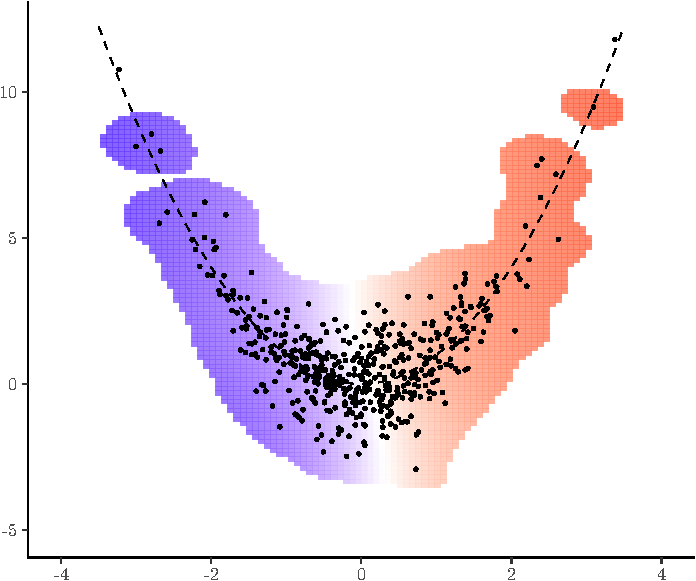
\includegraphics[width=0.49\linewidth]{figures/structural-plot-1} }
    \subfloat[The estimated LGPC along the curve $X_2 = X_1^2$ with 95\% confidence band.\label{fig:structural-plot2}]{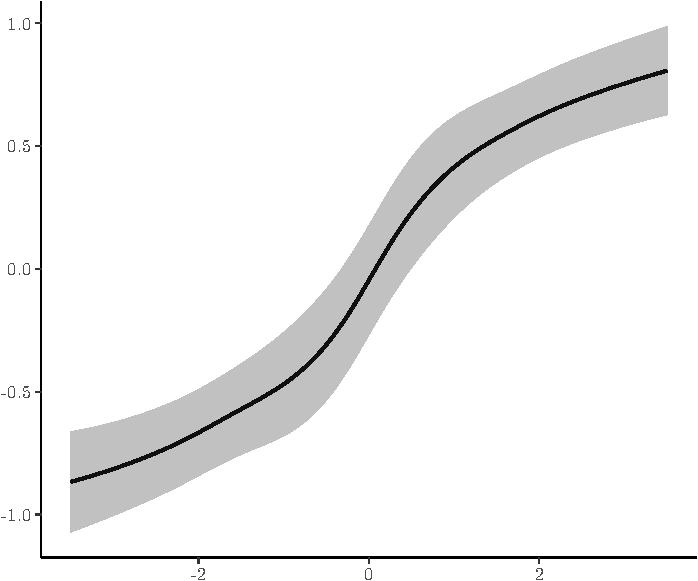
\includegraphics[width=0.49\linewidth]{figures/structural-plot-2} }
    \caption{The structural model. The fully trivariate model of Section 3.1.1 is used.}\label{fig:structural-plot}
\end{figure}

\begin{equation}
X_2 = X_1^2 + X_3,
\label{eq:structural}
\end{equation}
where we observe all components in \((X_1, X_2, X_3)\). There is, obviously, a strong dependence between \(X_1\) and \(X_2\), and furthermore, this dependence is deterministic when conditioning on \(X_3 = x_3\). It is, however, well known that \(X_1\) and \(X_1^2 + x_3\) are uncorrelated if \(\E(X_1) = \E(X_1^3) = 0\), but the LGPC easily reveals conditional dependence between \(X_1\) and \(X_2\) in this case. Let us generate \(n = 500\) independent observations each from \(X_1 \sim \mathcal{N}(0,1)\) and \(X_3 \sim \mathcal{N}(0,1)\) and calculate \(X_2\) by \eqref{eq:structural}. The sample partial correlation between \(X_1\) and \(X_2\) is \(-0.037\) in this case, but the LGPC, which in this case is calculated using the simplified pairwise structure defined in Section 3.1.2, displayed in Figure \ref{fig:structural-plot1}, indicates strong departures from conditional independence on the plane defined by \(X_3 = 0\). Indeed, we identify a region of \emph{negative conditional relationship} on the left hand side of the plot, which makes good sense because small values of \(X_2\) is typically observed together with large values of \(X_1\) and vice versa. The opposite phenomenon is clearly visible in the right hand half of the plot. In Figure \ref{fig:structural-plot2} we have plotted the estimated LGPC along the curve \(X_2 = X_1^2\), along with an asymptotic 95\% confidence band. The full trivariate fit presented in Section 3.1.1 gives a very similar picture.

This points to an important feature of the LGPC, as we also saw in one of the simulated examples in the main article: It is able to \emph{distinguish between positive and negative conditional relationships}, which, to our knowledge, has until now not been possible beyond the linear and jointly Gaussian setting using the ordinary partial correlation.

\begin{figure}
\subfloat[Local partial dependence map of $V_t^*$ vs. $R_{t-1}$ \newline on the plane defined by $V_{t-1}^* = 0$\label{fig:realplots1}]{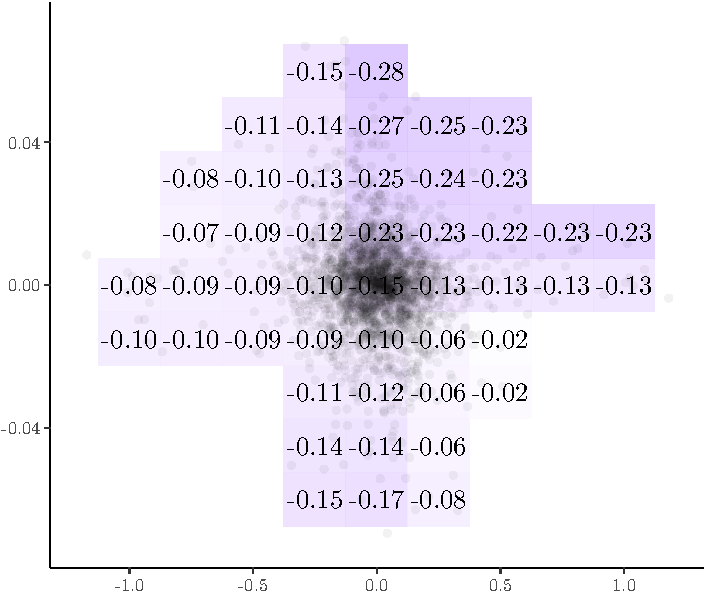
\includegraphics[width=0.49\linewidth]{figures/realplots-1} }
\subfloat[Local partial dependence map of $R_t$ vs. $V_{t-1}^*$ \newline on the plane defined by $R_{t-1} = 0$\label{fig:realplots2}]{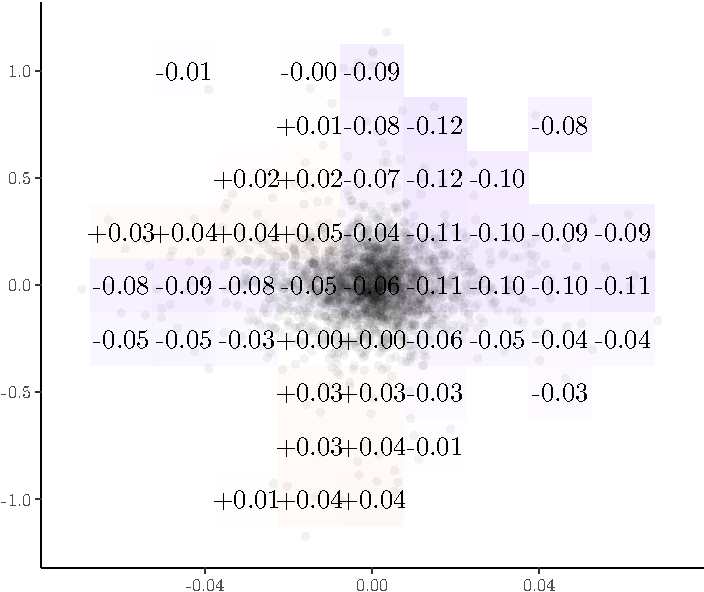
\includegraphics[width=0.49\linewidth]{figures/realplots-2} }\newline
\subfloat[Local partial dependence map of $R_t$ vs. $V_{t-1}^*$ \newline on the  plane defined by $R_{t-1} = -0.05$\label{fig:realplots3}]{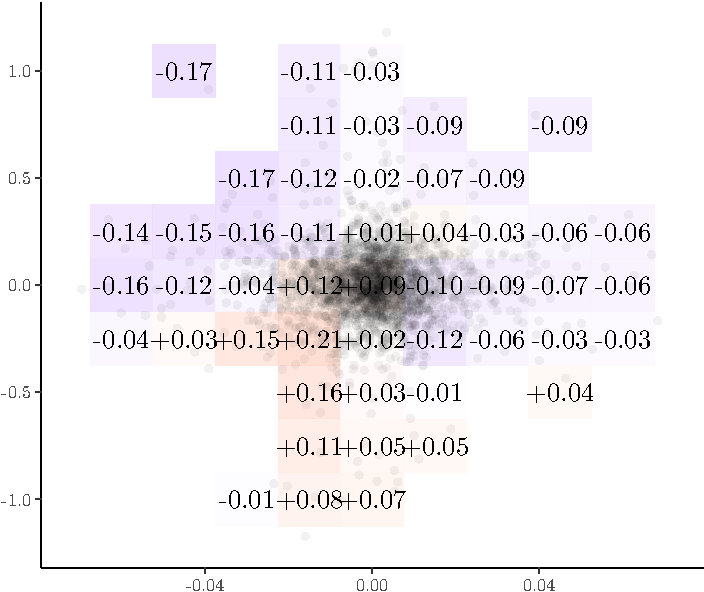
\includegraphics[width=0.49\linewidth]{figures/realplots-3} }
\subfloat[Local partial dependence map of $R_t$ vs. $V_{t-1}^*$ \newline on the  plane defined by $R_{t-1} = 0.05$\label{fig:realplots4}]{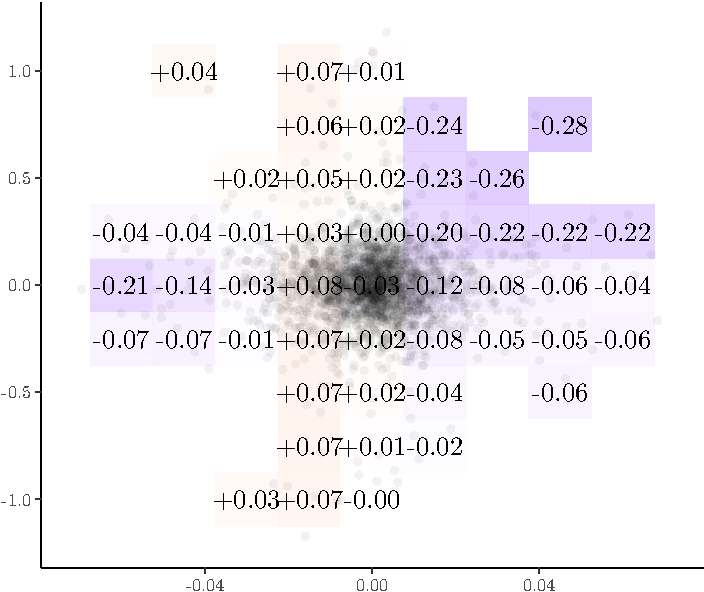
\includegraphics[width=0.49\linewidth]{figures/realplots-4} }
\caption{Local partial dependence maps for the S\&P 500 data}\label{fig:realplots}
\end{figure}

Let us briefly demonstrate a practical implementation of the LGPC in another situation involving real data. As in the empirical example in the main article, we look at Granger causality.

One fairly recent method for testing for Granger causality is based on the maximal conditional correlation and was introduced by Huang (\protect\hyperlink{ref-huang2010testing}{2010}) and later extended to the time series case by Cheng and Huang (\protect\hyperlink{ref-cheng2012conditional}{2012}). The latter authors use this test to examine whether trading volume Granger caused index value, or vice versa, on the S\&P 500 stock index during the first decade of this century. Using the daily price series \(\{P_t\}\) and volume \(\{V_t\}\) they define the log-differenced series

\[R_t = 100\log\left(\frac{P_t}{P_{t-1}}\right) \,\,\, \textrm{ and } \,\,\, V_t^* = \log\left(\frac{V_t}{V_{t-1}}\right).\]
Further, they denote by \(R_{t-1} \not\Rightarrow V_t^*\) the Granger non-causality from \(\{R_t\}\) to \(\{V_t^*\}\), which they analyze by putting the following null hypothesis to the test:

\begin{equation}
\textrm{H}_0: V_t^* \perp R_{t-1} \,\, | \,\, V_{t-1}^*.
\label{eq:grangernull500}
\end{equation}

Granger non-causality in the opposite direction, \(V_{t-1}^* \not\Rightarrow R_t\) is formulated and tested for in the obvious way.

A linear test rejects \(R_{t-1} \not\Rightarrow V_t^*\), but not \(V_{t-1}^* \not\Rightarrow R_t\). The nonparametric test by Cheng and Huang (\protect\hyperlink{ref-cheng2012conditional}{2012}) rejects both, leading to the natural conclusion that there are nonlinear relationships in the latter situation that remain unseen by linear models. What is it, though, in this particular data set, that leads to such results? Estimates of the local partial Gaussian correlation provide some clues towards answering that question.

We obtain daily observations on price and trading volume on the S\&P 500 index from January 1st 2000 until December 31st 2009 from Yahoo Finance (\protect\hyperlink{ref-yahoo}{2018}), and plot the estimated trivariate LGPC between \(V_t^*\) and \(R_{t-1}\) on the plane defined by \(V_{t-1}^* = 0\) in Figure \ref{fig:realplots1}. Departures from \(\alpha(V_t^*, R_{t-1}) \equiv 0\) provide evidence against \(R_{t-1} \not\Rightarrow V_{t}^*\). Similarly, we plot the estimated LGPC between \(R_t\) and \(V^*_{t-1}\) on the plane \(R_{t-1} = 0\) in Figure \ref{fig:realplots2} in which departures from \(\alpha(R_t, V^*_{t-1}) \equiv 0\) provide evidence against \(V^*_{t-1} \not\Rightarrow R_t\). We have used a proportionality constant of \(c = 3.5\) to calculate the estimates (see discussion on bandwidth selection in Section 4 of the main article). The observations can be seen in the background of both plots.

The differences between Figures \ref{fig:realplots1} and \ref{fig:realplots2} are subtle, but important. In Figure \ref{fig:realplots1}, \(\widehat\alpha(V_t^*, R_{t-1})\) is mostly negative, especially in the data rich portions of the sample space (other values of the conditioning variable \(V_{t-1}^*\) than zero give similar pictures). Indeed, the \emph{global} partial correlation in this situation is \(\widehat{\alpha}_{\textrm{glob}} = -0.086\), which is significantly different from zero. The global partial correlation in the second situation is very small though: \(\widehat{\alpha}_{\textrm{glob}} = -0.0018\), but Figure \ref{fig:realplots2} still reveals departures from conditional independence of similar magnitudes as in Figure \ref{fig:realplots1}. The difference is that the estimated LGPC is positive (primarily in the second and fourth quadrants) as well as negative (in the first and third quadrants), but this pattern collapses to the constant global value \(\alpha(R_t, V_{t-1}^*) = \alpha_{\textrm{glob}} \approx 0\) as the bandwidths tend to infinity. In Figures \ref{fig:realplots3} and \ref{fig:realplots4} we can explore the conditional dependence between \(R_t\) and \(V_{t-1}\) at high and low levels of \(R_{t-1}\), respectively, and we see even more clear differences in this dimension, especially in the first and second quadrants.

The \(p\)-values for tests of the hypothesis \eqref{eq:grangernull500} and its opposite counterpart, using our new test for conditional independence as presented in the next section and with \(c\)-values for the bandwidth as chosen there, are both equal to 0.

\hypertarget{power-studies}{%
\section{POWER STUDIES}\label{power-studies}}

Table 2\(^*\) below is the extended version of Table 2 in the main article, sample size is \(n=100\):

\vspace{1cm}



\renewcommand{\arraystretch}{1.2}
\begin{table}[h]
\resizebox{\textwidth}{!}{%
\begin{tabular}{l|rrrr|rrrrrr}
\toprule
&\multicolumn{4}{c}{Level} & \multicolumn{6}{c}{Power} \\
$\downarrow$ Test $\mid$ DGP $\rightarrow$ & 1 & 2 & 3 & 4 & 5 & 6 & 7 & 8 & 9 & 10 \\
\midrule
CHF&\texttt{0.034}&\texttt{0.058}&\texttt{-}&\texttt{-}&\texttt{0.780}&\texttt{0.792}&\texttt{0.520}&\texttt{0.780}&\texttt{0.728}&\texttt{0.580}\\
CM&\texttt{0.054}&\texttt{0.058}&\texttt{0.060}&\texttt{0.048}&\texttt{0.920}&\texttt{0.548}&\texttt{0.504}&\texttt{0.412}&\texttt{0.384}&\texttt{0.188}\\
HEL, $\scriptstyle c = 1$&\texttt{0.096}&\texttt{0.060}&\texttt{0.048}&\texttt{0.072}&\texttt{0.668}&\texttt{0.756}&\texttt{0.388}&\texttt{0.860}&\texttt{0.828}&\texttt{0.680}\\
HEL, $\scriptstyle c = 1.5$&\texttt{0.068}&\texttt{0.056}&\texttt{0.052}&\texttt{0.056}&\texttt{0.888}&\texttt{0.940}&\texttt{0.512}&\texttt{0.924}&\texttt{0.952}&\texttt{0.812}\\
HEL, $\scriptstyle c = 2$&\texttt{0.072}&\texttt{0.036}&\texttt{0.072}&\texttt{0.048}&\texttt{0.952}&\texttt{\underline{0.944}}&\texttt{0.576}&\texttt{0.940}&\texttt{\underline{0.988}}&\texttt{\underline{0.912}}\\
KS&\texttt{0.042}&\texttt{0.056}&\texttt{0.056}&\texttt{0.040}&\texttt{0.780}&\texttt{0.404}&\texttt{0.380}&\texttt{0.288}&\texttt{0.292}&\texttt{0.156}\\
\rowcolor{Gray}LGPC, $\scriptstyle c = 1.0$&\texttt{0.054}&\texttt{0.048}&\texttt{0.046}&\texttt{0.046}&\texttt{0.910}&\texttt{0.722}&\texttt{0.559}&\texttt{\underline{0.990}}&\texttt{0.968}&\texttt{0.866}\\
\rowcolor{Gray}LGPC, $\scriptstyle c = 1.4$&\texttt{0.047}&\texttt{0.043}&\texttt{0.046}&\texttt{0.047}&\texttt{0.971}&\texttt{0.855}&\texttt{0.727}&\texttt{0.969}&\texttt{0.916}&\texttt{0.765}\\
LIN&\texttt{0.044}&\texttt{0.061}&\texttt{0.050}&\texttt{0.060}&\texttt{\underline{0.999}}&\texttt{0.337}&\texttt{0.213}&\texttt{0.126}&\texttt{0.163}&\texttt{0.153}\\
MCC, $\scriptstyle c = 1$&\texttt{0.046}&\texttt{0.050}&\texttt{0.050}&\texttt{0.047}&\texttt{0.746}&\texttt{0.717}&\texttt{0.400}&\texttt{0.873}&\texttt{0.566}&\texttt{0.320}\\
MCC, $\scriptstyle c = 1.5$&\texttt{0.040}&\texttt{0.052}&\texttt{0.056}&\texttt{0.055}&\texttt{0.814}&\texttt{0.779}&\texttt{0.329}&\texttt{0.889}&\texttt{0.618}&\texttt{0.341}\\
MCC, $\scriptstyle c = 2$&\texttt{0.041}&\texttt{0.050}&\texttt{0.053}&\texttt{0.062}&\texttt{0.852}&\texttt{0.793}&\texttt{0.218}&\texttt{0.860}&\texttt{0.631}&\texttt{0.348}\\
SCM&\texttt{0.076}&\texttt{0.060}&\texttt{0.084}&\texttt{0.064}&\texttt{0.924}&\texttt{0.464}&\texttt{0.352}&\texttt{0.500}&\texttt{0.224}&\texttt{0.196}\\
SEL&\texttt{0.054}&\texttt{0.038}&\texttt{-}&\texttt{-}&\texttt{0.840}&\texttt{0.856}&\texttt{\underline{0.760}}&\texttt{0.904}&\texttt{0.716}&\texttt{0.556}\\
SKS&\texttt{0.064}&\texttt{0.056}&\texttt{0.088}&\texttt{0.068}&\texttt{0.728}&\texttt{0.236}&\texttt{0.288}&\texttt{0.340}&\texttt{0.120}&\texttt{0.112}\\
\bottomrule
\end{tabular}}
\caption*{Table 2$^*$: Level and power, $n = 100$. This is the full version of Table 2 in the main article}
\label{tab:n100}
\end{table}






\newpage

In Table 3\(^*\) we present level and power results for various conditional independence tests applied to the DGPs listed in Table 1 in the paper for sample size \(n = 200\):

\renewcommand{\arraystretch}{1.2}
\begin{table}[h]
\resizebox{\textwidth}{!}{%
\begin{tabular}{l|rrrr|rrrrrr}
\toprule
&\multicolumn{4}{c}{Level} & \multicolumn{6}{c}{Power} \\
$\downarrow$ Test $\mid$ DGP $\rightarrow$ & 1 & 2 & 3 & 4 & 5 & 6 & 7 & 8 & 9 & 10 \\
\midrule
BRT, $\scriptstyle c = 1$&\texttt{0.037}&\texttt{0.025}&\texttt{0.028}&\texttt{0.032}&\texttt{0.995}&\texttt{0.996}&\texttt{\underline{0.979}}&\texttt{0.989}&\texttt{0.904}&\texttt{0.785}\\
BRT, $\scriptstyle c = 1.5$&\texttt{0.044}&\texttt{0.025}&\texttt{0.025}&\texttt{0.037}&\texttt{0.971}&\texttt{0.993}&\texttt{0.931}&\texttt{0.997}&\texttt{0.931}&\texttt{0.759}\\
BRT, $\scriptstyle c = 2$&\texttt{0.064}&\texttt{0.023}&\texttt{0.023}&\texttt{0.052}&\texttt{0.943}&\texttt{0.979}&\texttt{0.873}&\texttt{0.997}&\texttt{0.912}&\texttt{0.728}\\
BT, $\scriptstyle c_1 = 1, c_2 = 1$&\texttt{0.047}&\texttt{0.051}&\texttt{0.041}&\texttt{0.053}&\texttt{0.996}&\texttt{0.812}&\texttt{0.852}&\texttt{\underline{1.000}}&\texttt{0.936}&\texttt{-}\\
BT, $\scriptstyle c_1 = 0.85, c_2 = 0.7$&\texttt{0.048}&\texttt{0.044}&\texttt{0.064}&\texttt{0.056}&\texttt{0.988}&\texttt{0.728}&\texttt{0.792}&\texttt{\underline{1.000}}&\texttt{0.908}&\texttt{-}\\
BT, $\scriptstyle c_1 = 0.75, c_2 = 0.6$&\texttt{0.036}&\texttt{0.048}&\texttt{0.052}&\texttt{0.052}&\texttt{0.976}&\texttt{0.719}&\texttt{0.808}&\texttt{\underline{1.000}}&\texttt{0.896}&\texttt{-}\\
CHF&\texttt{0.046}&\texttt{0.042}&\texttt{-}&\texttt{-}&\texttt{0.976}&\texttt{0.988}&\texttt{0.820}&\texttt{0.952}&\texttt{0.944}&\texttt{0.864}\\
CM&\texttt{0.044}&\texttt{0.056}&\texttt{0.060}&\texttt{0.048}&\texttt{0.992}&\texttt{0.740}&\texttt{0.788}&\texttt{0.680}&\texttt{0.476}&\texttt{0.360}\\
HEL, $\scriptstyle c = 1$&\texttt{0.064}&\texttt{0.052}&\texttt{0.080}&\texttt{0.080}&\texttt{0.900}&\texttt{0.960}&\texttt{0.596}&\texttt{0.992}&\texttt{0.968}&\texttt{0.880}\\
HEL, $\scriptstyle c = 1.5$&\texttt{0.064}&\texttt{0.056}&\texttt{0.048}&\texttt{0.036}&\texttt{0.980}&\texttt{\underline{1.000}}&\texttt{0.808}&\texttt{0.992}&\texttt{0.972}&\texttt{0.972}\\
HEL, $\scriptstyle c = 2$&\texttt{0.044}&\texttt{0.060}&\texttt{0.056}&\texttt{0.048}&\texttt{\underline{1.000}}&\texttt{\underline{1.000}}&\texttt{0.864}&\texttt{\underline{1.000}}&\texttt{\underline{1.000}}&\texttt{\underline{0.996}}\\
KS&\texttt{0.068}&\texttt{0.053}&\texttt{0.048}&\texttt{0.084}&\texttt{0.952}&\texttt{0.552}&\texttt{0.660}&\texttt{0.532}&\texttt{0.336}&\texttt{0.284}\\
\rowcolor{Gray}LGPC, $\scriptstyle c = 1.0$&\texttt{0.039}&\texttt{0.052}&\texttt{0.054}&\texttt{0.054}&\texttt{0.995}&\texttt{0.948}&\texttt{0.818}&\texttt{\underline{1.000}}&\texttt{\underline{1.000}}&\texttt{0.985}\\
\rowcolor{Gray}LGPC, $\scriptstyle c = 1.4$&\texttt{0.042}&\texttt{0.057}&\texttt{0.058}&\texttt{0.042}&\texttt{\underline{1.000}}&\texttt{0.993}&\texttt{0.956}&\texttt{\underline{1.000}}&\texttt{\underline{1.000}}&\texttt{0.958}\\
LIN&\texttt{0.043}&\texttt{0.053}&\texttt{0.042}&\texttt{0.050}&\texttt{\underline{1.000}}&\texttt{0.354}&\texttt{0.250}&\texttt{0.113}&\texttt{0.172}&\texttt{0.143}\\
MCC, $\scriptstyle c = 1$&\texttt{0.049}&\texttt{0.051}&\texttt{0.057}&\texttt{0.054}&\texttt{0.982}&\texttt{0.983}&\texttt{0.831}&\texttt{\underline{1.000}}&\texttt{0.947}&\texttt{0.679}\\
MCC, $\scriptstyle c = 1.5$&\texttt{0.046}&\texttt{0.048}&\texttt{0.049}&\texttt{0.053}&\texttt{0.995}&\texttt{0.989}&\texttt{0.872}&\texttt{\underline{1.000}}&\texttt{0.968}&\texttt{0.738}\\
MCC, $\scriptstyle c = 2$&\texttt{0.045}&\texttt{0.045}&\texttt{0.047}&\texttt{0.057}&\texttt{0.997}&\texttt{0.995}&\texttt{0.735}&\texttt{\underline{1.000}}&\texttt{0.971}&\texttt{0.745}\\
SCM&\texttt{0.048}&\texttt{0.060}&\texttt{0.064}&\texttt{0.068}&\texttt{0.980}&\texttt{0.648}&\texttt{0.620}&\texttt{0.720}&\texttt{0.352}&\texttt{0.280}\\
SEL&\texttt{0.052}&\texttt{0.033}&\texttt{-}&\texttt{-}&\texttt{0.992}&\texttt{\underline{1.000}}&\texttt{0.972}&\texttt{\underline{1.000}}&\texttt{0.884}&\texttt{0.864}\\
SKS&\texttt{0.056}&\texttt{0.028}&\texttt{0.064}&\texttt{0.072}&\texttt{0.964}&\texttt{0.324}&\texttt{0.512}&\texttt{0.552}&\texttt{0.148}&\texttt{0.136}\\
\bottomrule
\end{tabular}}
\caption*{Table 3$^*$: Level and power of conditional independence tests, $n = 200$}
\label{tab:n200}
\end{table}






Su and White (\protect\hyperlink{ref-su2014testing}{2014}) define two extensions to a subset of the data generating processes defined in Table 1 in which the conditioning variable \(\X_3\) is a vector with two and three components respectively. The first extension turns the conditioning variable \(\X_{3,t}\) in DGP1-DGP2 and DGP5-DGP10 \(X_{3,t}\) into a bivariate vector, where we define DGP1\(^{\prime}\) in the same way as before,

\begin{itemize}
\item[1$^{\prime}$.] $(X_{1,t}, X_{2,t}, \X_{3,t}) = (\epsilon_{1,t}, \epsilon_{2,t}, \fepsilon_{3,t})$,
\end{itemize}

but where \(\fepsilon_{3,t} \sim \mathcal{N}(0, \bm{I}_2)\), and where we define DGP2\(^{\prime}\) and DGP5\(^{\prime}\)-DGP10\(^{\prime}\) by setting \(\X_{3,t} = (X_{1, t-1}, X_{1, t-2})\), keeping \(X_{2,t}\) as before, and,

\begin{itemize}
\tightlist
\item[2$^{\prime}$.] $X_{1,t} = 0.5X_{1,t-1} + 0.25X_{1, t-2} + \epsilon_{1,t}$,
\item[5$^{\prime}$.] $X_{1,t} = 0.5X_{1,t-1} + 0.25X_{1, t-2} + 0.5X_{2,t} + \epsilon_{1,t}$,
\item[6$^{\prime}$.] $X_{1,t} = 0.5X_{1,t-1} + 0.25X_{1, t-2} + 0.5X_{2,t}^2 + \epsilon_{1,t}$,
\item[7$^{\prime}$.] $X_{1,t} = 0.5X_{1,t-1}X_{2, t} + 0.25X_{1,t-2}+ \epsilon_{1,t}$,
\item[8$^{\prime}$.] $X_{1,t} = 0.5X_{1,t-1} + 0.25X_{1,t-2} + 0.5X_{2, t}\epsilon_{1,t}$,
\item[9$^{\prime}$.] $X_{1,t} = \sqrt{h_t}\epsilon_{1,t}$, $h_t = 0.01 + 0.5X_{1,t-1}^2 + 0.25X_{1,t-2}^2 + 0.25X_{2,t}^2$, and
\item[10$^{\prime}$.] Same as DGP10 above, except for the new definition of $\X_{3,t}$.
\end{itemize}

We report the level and power results obtained by Su and White (\protect\hyperlink{ref-su2014testing}{2014}) for the methods CHF, CM, KS and SEL on these data by testing the null hypothesis
\[\textrm{H}_0: X_{t,1} \perp X_{t,2} \,\, | \,\, \X_{t,3},\]
and include results from our new test based on the multivariate simplification of the LGPC as defined in Section 3.1.2 in table 4\(^*\). The results are quite acceptable and compares well with other nonparametric methods.

The second extension introduced by Su and White (\protect\hyperlink{ref-su2014testing}{2014}) increases the dimension of the conditioning variable \(\X_{3,t}\) once more, so that \(\fepsilon_{3,t} \sim \mathcal{N}(0, \bm{I}_3)\), and where DGP2\(^{\prime\prime}\) and DGP5\(^{\prime\prime}\)-DGP10\(^{\prime\prime}\) are defined by by setting \(\X_{3,t} = (X_{1, t-1}, X_{1, t-2}, X_{1, t-3})\), and,

\begin{itemize}
\tightlist
\item[2$^{\prime\prime}$.] $X_{1,t} = 0.5X_{1,t-1} + 0.25X_{1, t-2} + 0.125X_{1,t-3} + \epsilon_{1,t}$,
\item[5$^{\prime\prime}$.] $X_{1,t} = 0.5X_{1,t-1} + 0.25X_{1, t-2} + 0.125X_{1,t-3} + 0.5X_{2,t} + \epsilon_{1,t}$,
\item[6$^{\prime\prime}$.] $X_{1,t} = 0.5X_{1,t-1} + 0.25X_{1, t-2} + 0.125X_{1,t-3} + 0.5X_{2,t}^2 + \epsilon_{1,t}$,
\item[7$^{\prime\prime}$.] $X_{1,t} = 0.5X_{1,t-1}X_{2, t} + 0.25X_{1,t-2} + 0.125X_{1,t-3} + \epsilon_{1,t}$,
\item[8$^{\prime\prime}$.] $X_{1,t} = 0.5X_{1,t-1} + 0.25X_{1,t-2} + 0.125X_{1,t-3} + 0.5X_{2, t}\epsilon_{1,t}$,
\item[9$^{\prime\prime}$.] $X_{1,t} = \sqrt{h_t}\epsilon_{1,t}$, $h_t = 0.01 + 0.5X_{1,t-1}^2 + 0.25X_{1,t-2}^2 + 0.125X_{1,t-3}^2 + 0.25X_{2,t}^2$, and
\item[10$^{\prime\prime}$.] Same as DGP10 and DGP10$^{\prime}$ above, except for the new definition of $\X_{3,t}$.
\end{itemize}
\renewcommand{\arraystretch}{1.1}
\begin{table}[hp]
\resizebox{\textwidth}{!}{%
\begin{tabular}{ll|rr|rrrrrr}
\toprule
&&\multicolumn{2}{c}{Level} & \multicolumn{6}{c}{Power} \\
Sample size & $\downarrow$ Test $\mid$ DGP $\rightarrow$ & 1$^{\prime}$ & 2$^{\prime}$ & 5$^{\prime}$ & 6$^{\prime}$ & 7$^{\prime}$ & 8$^{\prime}$ & 9$^{\prime}$ & 10$^{\prime}$ \\
\midrule
&&&&&&&&& \\ 
$n = 100$ & CHF&\texttt{0.028}&\texttt{0.042}&\texttt{0.720}&\texttt{0.704}&\texttt{0.412}&\texttt{0.564}&\texttt{\underline{0.460}}&\texttt{\underline{0.556}}\\
&CM&\texttt{0.028}&\texttt{0.016}&\texttt{0.656}&\texttt{0.360}&\texttt{0.108}&\texttt{0.512}&\texttt{0.164}&\texttt{0.208}\\
&KS&\texttt{0.040}&\texttt{0.020}&\texttt{0.400}&\texttt{0.284}&\texttt{0.056}&\texttt{0.380}&\texttt{0.124}&\texttt{0.176}\\
\rowcolor{Gray}&LGPC, $\scriptstyle c = 1.75$&\texttt{0.048}&\texttt{0.033}&\texttt{\underline{0.951}}&\texttt{0.668}&\texttt{0.294}&\texttt{0.517}&\texttt{0.406}&\texttt{0.538}\\
&SEL&\texttt{0.052}&\texttt{0.040}&\texttt{0.844}&\texttt{\underline{0.828}}&\texttt{\underline{0.620}}&\texttt{\underline{0.568}}&\texttt{0.440}&\texttt{0.528}\\
&&&&&&&&& \\ 
$n = 200$ & CHF&\texttt{0.030}&\texttt{0.040}&\texttt{0.948}&\texttt{0.944}&\texttt{0.748}&\texttt{0.828}&\texttt{\underline{0.724}}&\texttt{\underline{0.860}}\\
&CM&\texttt{0.050}&\texttt{0.032}&\texttt{0.940}&\texttt{0.588}&\texttt{0.304}&\texttt{0.792}&\texttt{0.304}&\texttt{0.364}\\
&KS&\texttt{0.046}&\texttt{0.024}&\texttt{0.776}&\texttt{0.432}&\texttt{0.168}&\texttt{0.696}&\texttt{0.216}&\texttt{0.284}\\
\rowcolor{Gray}&LGPC, $\scriptstyle c = 1.75$&\texttt{0.059}&\texttt{0.035}&\texttt{\underline{0.998}}&\texttt{0.923}&\texttt{0.415}&\texttt{0.769}&\texttt{0.698}&\texttt{0.833}\\
&SEL&\texttt{0.058}&\texttt{0.026}&\texttt{0.972}&\texttt{\underline{0.988}}&\texttt{\underline{0.932}}&\texttt{\underline{0.832}}&\texttt{0.684}&\texttt{0.832}\\
&&&&&&&&& \\ 
$n = 400$ & CHF&\texttt{0.040}&\texttt{0.036}&\texttt{\underline{1.000}}&\texttt{0.984}&\texttt{0.972}&\texttt{0.996}&\texttt{0.920}&\texttt{\underline{0.984}}\\
&CM&\texttt{0.056}&\texttt{0.024}&\texttt{\underline{1.000}}&\texttt{0.884}&\texttt{0.552}&\texttt{0.980}&\texttt{0.556}&\texttt{0.668}\\
&KS&\texttt{0.060}&\texttt{0.024}&\texttt{\underline{1.000}}&\texttt{0.732}&\texttt{0.324}&\texttt{0.952}&\texttt{0.384}&\texttt{0.524}\\
\rowcolor{Gray}&LGPC, $\scriptstyle c = 1.75$&\texttt{0.048}&\texttt{0.018}&\texttt{\underline{1.000}}&\texttt{0.996}&\texttt{0.584}&\texttt{0.960}&\texttt{\underline{0.928}}&\texttt{0.978}\\
&SEL&\texttt{0.040}&\texttt{0.030}&\texttt{\underline{1.000}}&\texttt{\underline{1.000}}&\texttt{\underline{1.000}}&\texttt{\underline{1.000}}&\texttt{0.836}&\texttt{0.884}\\
\bottomrule
\end{tabular}}
\caption*{Table 4$^*$: Level and power, 4-dimensional data}
\label{tab:dim4}
\end{table}
\renewcommand{\arraystretch}{1.1}
\begin{table}[hp]
\resizebox{\textwidth}{!}{%
\begin{tabular}{ll|rr|rrrrrr}
\toprule
&&\multicolumn{2}{c}{Level} & \multicolumn{6}{c}{Power} \\
Sample size & $\downarrow$ Test $\mid$ DGP $\rightarrow$ & 1$^{\prime\prime}$ & 2$^{\prime\prime}$ & 5$^{\prime\prime}$ & 6$^{\prime\prime}$ & 7$^{\prime\prime}$ & 8$^{\prime\prime}$ & 9$^{\prime\prime}$ & 10$^{\prime\prime}$ \\
\midrule
&&&&&&&&& \\ 
\rowcolor{Gray}$n = 100$ & LGPC, $\scriptstyle c = 1.75$&\texttt{0.068}&\texttt{0.049}&\texttt{\underline{0.911}}&\texttt{\underline{0.567}}&\texttt{\underline{0.295}}&\texttt{\underline{0.266}}&\texttt{\underline{0.380}}&\texttt{\underline{0.521}}\\
&&&&&&&&& \\ 
$n = 200$ & CHF&\texttt{0.028}&\texttt{0.022}&\texttt{0.964}&\texttt{0.952}&\texttt{0.668}&\texttt{\underline{0.852}}&\texttt{\underline{0.552}}&\texttt{\underline{0.856}}\\
&CM&\texttt{0.050}&\texttt{0.028}&\texttt{0.756}&\texttt{0.484}&\texttt{0.192}&\texttt{0.788}&\texttt{0.260}&\texttt{0.448}\\
&KS&\texttt{0.048}&\texttt{0.032}&\texttt{0.500}&\texttt{0.380}&\texttt{0.096}&\texttt{0.660}&\texttt{0.212}&\texttt{0.372}\\
\rowcolor{Gray}&LGPC, $\scriptstyle c = 1.75$&\texttt{0.062}&\texttt{0.050}&\texttt{0.993}&\texttt{0.776}&\texttt{0.388}&\texttt{0.363}&\texttt{0.545}&\texttt{0.794}\\
&SEL&\texttt{0.056}&\texttt{0.026}&\texttt{\underline{0.996}}&\texttt{\underline{0.980}}&\texttt{\underline{0.860}}&\texttt{0.816}&\texttt{0.344}&\texttt{0.680}\\
&&&&&&&&& \\ 
$n = 400$ & CHF&\texttt{0.032}&\texttt{0.034}&\texttt{\underline{1.000}}&\texttt{0.972}&\texttt{0.928}&\texttt{0.884}&\texttt{\underline{0.792}}&\texttt{\underline{0.972}}\\
&CM&\texttt{0.050}&\texttt{0.032}&\texttt{0.992}&\texttt{0.728}&\texttt{0.400}&\texttt{\underline{0.912}}&\texttt{0.390}&\texttt{0.620}\\
&KS&\texttt{0.044}&\texttt{0.036}&\texttt{0.840}&\texttt{0.552}&\texttt{0.220}&\texttt{0.880}&\texttt{0.306}&\texttt{0.568}\\
\rowcolor{Gray}&LGPC, $\scriptstyle c = 1.75$&\texttt{0.048}&\texttt{0.030}&\texttt{\underline{1.000}}&\texttt{0.938}&\texttt{0.519}&\texttt{0.538}&\texttt{0.740}&\texttt{0.956}\\
&SEL&\texttt{0.056}&\texttt{0.038}&\texttt{\underline{1.000}}&\texttt{\underline{1.000}}&\texttt{\underline{1.000}}&\texttt{0.888}&\texttt{0.616}&\texttt{0.876}\\
\bottomrule
\end{tabular}}
\caption*{Table 5$^*$: Level and power, 5-dimensional data}
\label{tab:dim5}
\end{table}


Again, we observe simulation results in Table 5\(^*\). Contrary to Su and White (\protect\hyperlink{ref-su2014testing}{2014}), we have also run our test for \(n=100\) which reveals that we can obtain some power also in that case. All in all, the simplified test based on the LGPC performs mostly on par with other non-parametric tests in this setting as well.

\newpage

\hypertarget{references}{%
\section*{REFERENCES}\label{references}}
\addcontentsline{toc}{section}{REFERENCES}

\hypertarget{refs}{}
\begin{cslreferences}
\leavevmode\hypertarget{ref-bill:2008}{}%
Billingsley, Patrick. 2008. \emph{Probability and Measure}. John Wiley \& Sons.

\leavevmode\hypertarget{ref-brockwell1991time}{}%
Brockwell, Peter J, and Richard A Davis. 2006. \emph{Time Series: Theory and Methods: Theory and Methods}. Springer.

\leavevmode\hypertarget{ref-cheng2012conditional}{}%
Cheng, Yu-Hsiang, and Tzee-Ming Huang. 2012. ``A Conditional Independence Test for Dependent Data Based on Maximal Conditional Correlation.'' \emph{Journal of Multivariate Analysis} 107: 210--26.

\leavevmode\hypertarget{ref-fan2008nonlinear}{}%
Fan, Jianqing, and Qiwei Yao. 2008. \emph{Nonlinear Time Series: Nonparametric and Parametric Methods}. Springer Science \& Business Media.

\leavevmode\hypertarget{ref-gonccalves2002bootstrap}{}%
Gonçalves, Si@articlelacal2017local, title=Local Gaussian autocorrelation and tests for serial independence, author=Lacal, Virginia and TjØstheim, Dag, journal=Journal of Time Series Analysis, volume=38, number=1, pages=51--71, year=2017, publisher=Wiley Online Library lvia, and Halbert White. 2002. ``The Bootstrap of the Mean for Dependent Heterogeneous Arrays.'' \emph{Econometric Theory} 18 (6): 1367--84.

\leavevmode\hypertarget{ref-gonccalves2004maximum}{}%
Gonçalves, Silvia, and Halbert White. 2004. ``Maximum Likelihood and the Bootstrap for Nonlinear Dynamic Models.'' \emph{Journal of Econometrics} 119 (1): 199--219.

\leavevmode\hypertarget{ref-hall1980martingale}{}%
Hall, P, and CC Heyde. 1980. ``Martingale Limit Theory and Its Applications, Acad.'' \emph{Press, New York}.

\leavevmode\hypertarget{ref-hjort1996locally}{}%
Hjort, Nils Lid, and MC Jones. 1996. ``Locally Parametric Nonparametric Density Estimation.'' \emph{The Annals of Statistics}, 1619--47.

\leavevmode\hypertarget{ref-huang2010testing}{}%
Huang, Tzee-Ming. 2010. ``Testing Conditional Independence Using Maximal Nonlinear Conditional Correlation.'' \emph{The Annals of Statistics} 38 (4): 2047--91.

\leavevmode\hypertarget{ref-joe1989estimation}{}%
Joe, Harry. 1989. ``Estimation of Entropy and Other Functionals of a Multivariate Density.'' \emph{Annals of the Institute of Statistical Mathematics} 41 (4): 683--97.

\leavevmode\hypertarget{ref-jordanger2017nonlinear}{}%
Jordanger, Lars Arne, and Dag Tjøstheim. 2020. ``Nonlinear Spectral Analysis: A Local Gaussian Approach.'' \emph{arXiv Preprint arXiv:1708.02166v4, Revised version submitted to the Journal of the American Statistical Association}.

\leavevmode\hypertarget{ref-lacal2017local}{}%
Lacal, Virginia, and Dag Tjøstheim. 2017. ``Local Gaussian Autocorrelation and Tests for Serial Independence.'' \emph{Journal of Time Series Analysis} 38 (1): 51--71.

\leavevmode\hypertarget{ref-lacal2018estimating}{}%
---------. 2018. ``Estimating and Testing Nonlinear Local Dependence Between Two Time Series.'' \emph{Journal of Business \& Economic Statistics}, 1--13.

\leavevmode\hypertarget{ref-otneim2017locally}{}%
Otneim, Håkon, and Dag Tjøstheim. 2017. ``The Locally Gaussian Density Estimator for Multivariate Data.'' \emph{Statistics and Computing} 27 (6): 1595--1616.

\leavevmode\hypertarget{ref-otneim2017conditional}{}%
---------. 2018. ``Conditional Density Estimation Using the Local Gaussian Correlation.'' \emph{Statistics and Computing} 28 (2): 303--21.

\leavevmode\hypertarget{ref-paparoditis2000local}{}%
Paparoditis, Efstathios, and Dimitris N Politis. 2000. ``The Local Bootstrap for Kernel Estimators Under General Dependence Conditions.'' \emph{Annals of the Institute of Statistical Mathematics} 52 (1): 139--59.

\leavevmode\hypertarget{ref-rio1995functional}{}%
Rio, Emmanuel. 1995. ``The Functional Law of the Iterated Logarithm for Stationary Strongly Mixing Sequences.'' \emph{The Annals of Probability}, 1188--1203.

\leavevmode\hypertarget{ref-schervish1995theory}{}%
Schervish, Mark J. 2012. \emph{Theory of Statistics}. Springer Science \& Business Media.

\leavevmode\hypertarget{ref-su2008nonparametric}{}%
Su, Liangjun, and Halbert White. 2008. ``A Nonparametric Hellinger Metric Test for Conditional Independence.'' \emph{Econometric Theory} 24 (4): 829--64.

\leavevmode\hypertarget{ref-su2014testing}{}%
---------. 2014. ``Testing Conditional Independence via Empirical Likelihood.'' \emph{Journal of Econometrics} 182 (1): 27--44.

\leavevmode\hypertarget{ref-terasvirta2010modelling}{}%
Teräsvirta, Timo, Dag Tjøstheim, and Clive W. J. Granger. 2010. \emph{Modelling Nonlinear Economic Time Series}. Oxford University Press.

\leavevmode\hypertarget{ref-tjostheim2013local}{}%
Tjøstheim, Dag, and Karl Ove Hufthammer. 2013. ``Local Gaussian Correlation: A New Measure of Dependence.'' \emph{Journal of Econometrics} 172 (1): 33--48.

\leavevmode\hypertarget{ref-van2007parameter}{}%
Van den Bos, Adriaan. 2007. \emph{Parameter Estimation for Scientists and Engineers}. John Wiley \& Sons.

\leavevmode\hypertarget{ref-wang2017characteristic}{}%
Wang, Xia, and Yongmiao Hong. 2018. ``Characteristic Function Based Testing for Conditional Independence: A Nonparametric Regression Approach.'' \emph{Econometric Theory} 34 (4): 815--49.

\leavevmode\hypertarget{ref-yahoo}{}%
Yahoo Finance. 2018. \emph{Accessed June 2018}.
\end{cslreferences}

\end{document}
